\newpage
\clearpage

\section{Desenvolvimento do Projeto}
\label{project}

Nos capítulos anteriores, analisamos como as Redes Neurais Convolucionais (CNNs) - Capítulo \ref{cnn} - provocaram mudanças significativas nas abordagens de segmentação, expandindo as possibilidades de obtenção de resultados mais precisos e melhorando o desempenho dos métodos convencionais de segmentação, conforme discutido nos Capítulos \ref{segment} e \ref{semantic}.

Entretanto, ainda existem questões não resolvidas relacionadas às potenciais melhorias que modificações específicas nas componentes destas redes podem proporcionar \citep{AsgariTaghanaki2021DeepReview}. Dentre esses componentes, particular atenção é dada às limitações das camadas de \textit{pooling} tradicionais \citep{Liu2019Multi-LevelNetworks, He2015SpatialRecognition}. Estas camadas têm duas tarefas principais: reduzir a dimensionalidade dos dados, a fim de diminuir a carga computacional do modelo e, simultaneamente, preservar as informações mais relevantes, principalmente as espaciais.

Neste contexto, o objetivo primordial deste trabalho é propor uma nova técnica de \textit{pooling} para CNNs, aplicando testes em CNNs convencionais, mas com ênfase na segmentação semântica com o modelo U-Net. A abordagem proposta visa manter as informações espaciais dos dados de entrada enquanto realiza a necessária redução de dimensionalidade, mas considerando uma visão global do mapa de atributos, algo que não ocorre com os métodos tradicionais de \textit{pooling}. Os resultados obtidos serão posteriormente comparados com aqueles produzidos pelos métodos de \textit{pooling} comumente utilizados.

Este capítulo trata detalhadamente dos materiais e métodos utilizados para a condução e avaliação da pesquisa, discutidos em profundidade na Seção \ref{project:matmet}. Enquanto a aplicação de métricas específicas para a avaliação dos resultados será discutida na Seção \ref{project:exp_result}.
% e uma breve revisão quanto aos trabalhos relacionados à pesquisa proposta será discorrida na Seção \ref{project:revision}.

Finalmente, vale citar que nesse capítulo será possível encontrar uma apresentação detalhada do novo método de \textit{pooling} proposto e seu impacto na performance das redes de aprendizado profundo.


\subsection{Materiais e Métodos}
\label{project:matmet}
Esta seção busca esclarecer sobre todos os recursos tecnológicos, \textit{hardwares} e abordagens metodológicas que foram empregados para suportar a consecução dos experimentos deste estudo (Seção \ref{project:techard}). Neste contexto, é essencial elucidar acerca das motivações e origens da técnica proposta com a extração de características (Seção \ref{project:feature_extraction}), bem como a implementação da nova técnica de \textit{pooling}, denominada BPCAPooling (Seção \ref{project:bpca}), aplicada em estruturas de CNNs. Além disso, a descrição dos conjuntos de dados utilizados fornece um embasamento sólido para compreender a motivação e a importância dos resultados obtidos ao longo das fases de desenvolvimento, treinamento, validação e teste (Seção \ref{project:dataset}).

Nesta mesma seção, procura-se detalhar a metodologia e as estratégias adotadas nos experimentos realizados. A abordagem de transferência de aprendizado, em particular, recebe destaque (Seção \ref{project:transf}). Tal técnica envolve a adaptação, ou o chamado \textit{fine-tuning}, de um pré-modelo treinado para operar especificamente na tarefa de interesse, iniciando o processo de aprendizagem a partir de uma configuração pré-definida de pesos, como foi citado na Seção \ref{cnn:augment}.

Além disso, é válida a discussão acerca do procedimento de aumento de dados (Seção \ref{project:augment}), adotado como uma medida para minimizar possíveis vieses nos modelos e potencializar sua capacidade de generalização \citep{Shorten2019ALearning}.

Por fim, na Seção \ref{project:change_pooling}, abordaremos as respectivas modificações realizadas na camada de \textit{pooling} dos modelos, que foram cruciais para a realização e a validação do experimento. O entendimento dessa sistematização se faz necessário para garantir a replicação das etapas pelos futuros pesquisadores da comunidade científica e proporcionar avanços consideráveis na área de visão computacional.

\subsubsection{Tecnologias e \textit{Hardware}}
\label{project:techard}
Um dos principais recursos tecnológicos utilizados neste trabalho é a linguagem de programação Python (versão 3.9.18) \citep{VanRossum2009PythonManual}. Esta linguagem interpretada de alto nível é amplamente reconhecida na comunidade científica, com uma vasta gama de bibliotecas disponíveis que facilitam o desenvolvimento de soluções tanto em aprendizado de máquina e redes neurais profundas, quanto em visão computacional \citep{Millman2011PythonEngineers, Perkel2015Programming:Python}.

Várias bibliotecas complementaram o Python no desenvolvimento deste projeto, especialmente aquelas projetadas para auxiliar na implementação de soluções de visão computacional, aprendizado de máquina e redes neurais. Destas, destaca-se o \textit{TensorFlow} (versão 2.13.0) \citep{MartinAbadi2015Systems} e \textit{Keras} (versão 2.13.1) \citep{Chollet2015Keras}, utilizados juntos como um \textit{framework} para modelar, treinar e testar redes neurais, bem como definir otimizadores, funções de custo e métricas de desempenho \citep{Geron2017Hands-onSystems, Chollet2021DeepPython}. O \textit{OpenCV} (versão 4.8.1) \citep{Bradski2000TheLibrary.}, uma biblioteca poderosa para o processamento de imagens e aplicações de visão computacional, também desempenhou um papel crucial na aplicação de filtros de imagens e na realização de testes manuais para afinar os métodos que utilizam aprendizado profundo. Adicionalmente, a biblioteca \textit{Numpy} (versão 1.22.3) \citep{Harris2020} foi fundamental para realizar cálculos matemáticos e manipulações matriciais \citep{Oliphant2007PythonComputing, VanDerWalt2011TheComputation}.

No que diz respeito ao \textit{hardware} empregado para a pesquisa e desenvolvimento deste projeto, os componentes de \textit{hardware}, tais como as placas de vídeo e os processadores, foram cruciais para o processamento de dados durante as fases de treinamento e validação dos modelos de aprendizado de máquina. Inicialmente, os ensaios foram realizados na plataforma de computação em nuvem Google Colab \citep{Bisong2019GoogleColaboratory}, que disponibilizava uma placa de vídeo Tesla T4 GPU e um processador Intel Xeon CPU. No entanto, devido à limitações de disponibilidade e considerações de custo financeiro, foi realizada a transição para um sistema físico equipado com um processador Intel Core i9-12900F CPU e uma placa de vídeo NVIDIA RTX 4090 GPU, o qual foi considerado para todos os resultados e testes descritos no presente trabalho.

Por fim, é importante ressaltar que todos os métodos desenvolvidos neste projeto com o objetivo de realizar a segmentação semântica foram disponibilizados nos repositórios Github do autor\footnote{Perfil Github do autor - \url{https://github.com/Lucs1590}} de modo \textit{open-source}, em conformidade com a licença Apache v2.0 \citep{Licenses}. A intenção é fomentar o crescimento acadêmico e de pesquisa, assim como facilitar futuras melhorias no campo de segmentação com o uso de camadas de \textit{pooling} personalizadas, como a camada BPCAPooling, que é detalhada na Seção \ref{project:bpca}.

\subsubsection{Extração de Características}
\label{project:feature_extraction}

Lidar com grandes conjuntos de dados nas redes neurais profundas é um desafio, pois a análise desses dados pode ser pesada devido à sua densidade ou à dimensionalidade elevada \citep{Liang2017TextReview}. Essa questão demanda um hardware robusto, pois quanto maior a quantidade e a dimensionalidade dos dados, maior é a exigência de poder computacional \citep{Benyahia2022Multi-featuresClassification}. A abordagem de extração de características é especialmente comum em ambientes de aprendizado baseado em texto, conforme discutido por \cite{Liang2017TextReview}, e se estende ao uso de convoluções em CNNs, como será abordado na Seção \ref{cnn:conv}.

Portanto, a extração de características surge como uma estratégia crucial para a redução da dimensionalidade, onde um conjunto inicial de dados brutos é transformado em grupos mais gerenciáveis para processamento \citep{Benyahia2022Multi-featuresClassification}. Esse processo frequentemente envolve a combinação ou seleção de variáveis, resultando em uma significativa redução na quantidade de dados a serem processados. Além disso, essas características ainda preservam a representatividade do conjunto original, sendo capazes de reduzir redundâncias para análises específicas.

Um exemplo de algoritmo capaz de agregar essas vantagens ao processo extração de características é o \textit{Principal Component Analysis} (PCA), que foi desenvolvido como uma técnica estatística de transformações ortogonais que almeja transformar um conjunto de variáveis correlacionadas em um conjunto linearmente de variáveis não correlacionadas, extraindo de um conjunto de dados as características essenciais \citep{Wold1987PrincipalAnalysis} e obtendo como resultado, um conjunto de dados menor, mas sem perdas em relação ao conjunto original.

O funcionamento do algoritmo de PCA para a extração de características pode ser resumido pelo passo-a-passo a seguir \citep{Song2010FeatureAnalysis}:

\begin{enumerate}
    \item Padronização dos dados, com a subtração da média $\boldsymbol{\mu}$ de todas as dimensões em relação ao valor de entrada inicial $\boldsymbol{z}$, dividido pelo desvio padrão $\sigma$, como descrito na Equação \ref{deep:eq:pca_1}:

    \begin{equation}
        \label{deep:eq:pca_1}
        \boldsymbol{z} = \frac{\boldsymbol{x} - \mu}{\sigma};
    \end{equation}

    \item Cálculo da matriz de covariância, com $X$ representando a primeira dimensão da entrada e $Y$ a segunda, conforme a Equação \ref{deep:eq:pca_2}:
    
    \begin{equation}
        \label{deep:eq:pca_2}
        \boldsymbol{A} = \text{cov}(X, Y) = \frac{1}{n-1} \sum_{i=1}^{n} (X_i - \bar{x}) (Y_i - \bar{y}),
    \end{equation}
    onde \(\bar{x}\) e \(\bar{y}\) representam as médias das variáveis $X$ e $Y$ respectivamente, e $n$ é o número de observações;

    \item Cálculo dos autovetores e autovalores correspondentes. Para a realização desse passo, o calculo dos autovetores em relação à matriz de covariância $\boldsymbol{A}$ pode ser representado pela Equação \ref{deep:eq:pca_3}:

    \begin{equation}
        \label{deep:eq:pca_3}
        \boldsymbol{A}\overrightarrow{v} = \lambda\overrightarrow{v},
    \end{equation}
    em que $\lambda$ representa um vetor de autovalores. O que significa que a transformação linear é definida por $\lambda$ e a equação pode ser transcrita pela Equação \ref{deep:eq:pca_4}:

        \begin{equation}
        \label{deep:eq:pca_4}
        \boldsymbol{A}\overrightarrow{v} - \lambda\overrightarrow{v} = 0
        \Rightarrow \overrightarrow{v}(\boldsymbol{A} - \lambda \boldsymbol{I}) = 0,
    \end{equation}
    tendo $I$ como uma matriz identidade.

    \item Escolha de $k$ autovetores com maiores autovalores, após realizar uma organização decrescente de autovalores, como demonstra a Equação \ref{deep:eq:pca_5}:

    \begin{equation}
        \label{deep:eq:pca_5}
        \boldsymbol{W}_k = \begin{bmatrix} \overrightarrow{v}_1 & \overrightarrow{v}_2 & \cdots & \overrightarrow{v}_k \end{bmatrix}.
    \end{equation}

    Nessa equação, $\boldsymbol{W}_k$ representa a matriz formada pelos $k$ autovetores correspondentes aos maiores autovalores selecionados após a organização decrescente dos autovalores. Cada autovetor $\overrightarrow{v}_i$ faz parte da matriz $\boldsymbol{W}_k$ e compõe as novas dimensões do conjunto de dados transformado, onde $k$ é o número desejado de bases para o novo conjunto de dados após a aplicação do PCA.

    
\end{enumerate}

Além disso, é importante mencionar que o PCA também pode ser obtido através do método de Decomposição em Valores Singulares (\textit{Singular Value Decomposition} - SVD) \citep{Stewart2006OnDecomposition}, o qual é utilizado para extrair os componentes principais do conjunto de dados de entrada.

Entre as vantagens do algoritmo PCA, destaca-se a eliminação das correlações entre as características, garantindo a independência entre os componentes principais e evitando viés em relação a características específicas. Além disso, o algoritmo melhora o desempenho e reduz o custo computacional ao diminuir as dimensões dos dados, especialmente útil ao lidar com conjuntos de dados de alta dimensionalidade. Finalmente, o PCA ajuda a reduzir problemas de superajustamento ao diminuir o número de características, mitigando os riscos associados a ter muitas variáveis e, frequentemente, facilita a visualização dos dados ao transformar dados de alta dimensão em uma forma de dimensão mais baixa e mais gerenciável, simplificando a compreensão dos dados.

No entanto, o PCA também apresenta desvantagens, como o fato de tornar os componentes gerados menos interpretáveis do que os dados originais, uma vez que os componentes principais gerados são combinações das características originais. Além disso, o PCA requer a padronização dos dados antes da implementação; sem isso, o algoritmo pode falhar em determinar os componentes principais ideais. Finalmente, embora o PCA busque capturar a máxima variância entre as características, uma seleção inadequada dos componentes principais pode resultar na perda de alguma informação em comparação com o conjunto original de características.

\subsubsection{\textit{Block-based Principal Component Analysis Pooling} (BPCAPooling)}
\label{project:bpca}
A técnica \textit{Block-based Principal Component Analysis} (BPCA) foi introduzida como uma variação do método convencional do \textit{Principal Component Analysis} (PCA) no trabalho de \cite{Salvadeo2011}, propondo um método que inicialmente foi utilizado para a extração de características de imagens como parte de uma \textit{pipeline} de reconhecimento de reconhecimento facial no conjunto de dados \textit{The AR Face Database}\footnote{\textit{AR Face Database Webpage} - \url{https://www2.ece.ohio-state.edu/~aleix/ARdatabase.html}} \citep{MartNez1998TheDatabase}, propondo um método de extração que trouxesse à análise menor custo computacional, redução de dimensionalidade e uma geometria de hiperespaço que fosse mais intuitiva, destacando o diferencial de que com esse método fosse possível preservar a espacialidade da informação.

O método proposto opera por meio da subdivisão de uma imagem em blocos $k \times k$, em que os blocos geralmente possuem tamanhos iguais (por exemplo, $3 \times 3$, $8 \times 8$, etc.). Em seguida, considerando cada bloco como uma amostra, o PCA é aplicado, sendo que cada um desses blocos são projetados no espaço do componente principal. Consequentemente, cada bloco $k \times k$ passa a ter um tamanho reduzido, definindo uma imagem com $r$ características (o mesmo número de blocos), posicionadas espacialmente nos respectivos blocos. Esse processo pode ser visualizado através da Figura \ref{project:fig:bpca_1}.

\begin{figure}[H]
    \centering
    \caption{Exemplo de aplicação do BPCA.}
    \label{project:fig:bpca_1}
    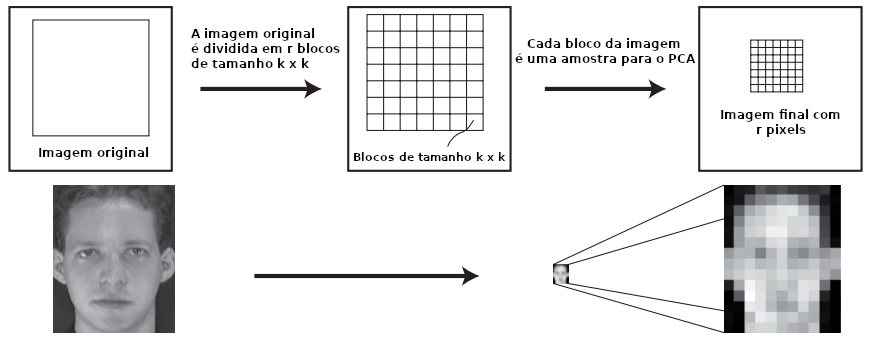
\includegraphics[width=1\textwidth]{recursos/imagens/project/BPCA.png}

    Fonte: retirado e adaptado de \cite{Salvadeo2011}.
\end{figure}

Ao contrário de uma combinação linear simples de amostras distintas, BPCA compõe uma representação organizada, formada por pequenos blocos do mapa de características original, conforme exibido na Imagem final com $r$ \textit{pixels} da Figura \ref{project:fig:bpca_1}. Esta técnica incorpora a teoria do PCA para realização do mapeamento não supervisionado visando a minimização do erro quadrático médio entre a entrada original e a apresentação projetada. Dessa forma, é possível sintetizar características essenciais da imagem de entrada numa representação compacta de maior relevância contextual \citep{Kuncheva2014PCAData}. Isso permite que a BPCA seja um componente eficaz ao enfrentar grandes volumes de dados, como é comum no âmbito de processamento de imagens.

As camadas de \textit{pooling} têm sido eficazes em CNNs para reduzir a dimensionalidade dos dados \citep{Paul2019DimensionalityPooling}. Neste trabalho, a inovação proposta é a aplicação da técnica BPCA como uma camada de \textit{pooling} - sendo nomeada de BPCAPooling - não mais para extração de características, conforme proposto originalmente por \cite{Salvadeo2011}, mas como uma estratégia para preservar a espacialidade da informação entre as camadas convolucionais, num olhar global para o mapa de atributos, associada ao benefício proposto pela técnica de minimização do erro quadrático médio entre a entrada e saída como uma camada de \textit{pooling}.

Essa camada de \textit{pooling} segue o processo original do BPCA, onde são extraídas informações principais de cada bloco, reduzindo a dimensionalidade dos dados e preservando características relevantes. Além disso, o método foi aprimorado pela normalização dos blocos utilizando média ($\mu$) e desvio padrão ($\sigma$). Na sequência, é aplicada a técnica de \textit{Singular Value Decomposition} (SVD) para extrair os componentes principais ($\text{{pca\_components}}$), como explicado na Seção \ref{project:feature_extraction}, e, finalmente, os blocos são transformados por meio da projeção nesses componentes selecionados. O resultado é um mapa de características menor em tamanho, porém, preservando informações essenciais ao concatenar os blocos transformados.

A formulação matemática do processo realizado pela camada de \textit{pooling} BPCAPooling pode ser representada pela Equação \ref{project:eq:bpca}:

\begin{equation}
    \label{project:eq:bpca}
    \begin{split}
        Y_{i,j,k} &= \text{BPCAPooling}(\boldsymbol{X}_{i',j',k'}) \\
                  &= \text{reshape}\left(\text{SVD}\left(\frac{{\boldsymbol{X} - \boldsymbol{\mu}}}{{\boldsymbol{\sigma}}}\right) \cdot \text{pca\_components}\right),
    \end{split}
\end{equation}
onde $\boldsymbol{X}$ é a imagem de entrada com $i'$ como altura de entrada, $j'$ como largura de entrada e $k'$ como número de canais de entrada; e $Y$ é a imagem de saída, com $i$ representando altura de saída, $j$ como largura de saída e $k$ como profundidade de saída (ou seja, o número de canais). Aqui, $\text{\textit{reshape}}$ reorganiza os blocos transformados para uma estrutura de saída apropriada, $\text{SVD}$ representa a decomposição em valores singulares dos blocos normalizados, $\boldsymbol{\mu}$ é o vetor médio dos blocos extraídos, $\boldsymbol{\sigma}$ é o vetor de desvio padrão dos blocos extraídos, e $\text{pca\_components}$ é uma matriz contendo os primeiros componentes principais selecionados.

Essa formulação matemática descreve o processo de \textit{pooling} realizado pela camada BPCAPooling, que extrai informações relevantes dos blocos de entrada, reduzindo sua dimensionalidade e preservando características importantes para o aprendizado eficiente da rede neural convolucional.

Quando se analisa a complexidade de uma função em notação Big O, que descreve o quão escalável é a função, pode-se expressá-la como $O(HWD * \min(P^2, ND))$ no pior caso. Isso é resultado da complexidade em cada um dos passos dos seguintes processos:

\begin{enumerate}
    \item Extração de \textit{patches} do mapa de características de entrada, de tamanho $(H,W,C)$, gerando \textit{patches} de dimensão $(P,P,D)$. Esse processo é representado pela notação $O(HWD * P^2)$;
    \item Normalização utilizando a média e o desvio padrão, com a notação $O(HWD)$;
    \item Aplicação da decomposição em valores singulares em uma matriz $(HWD, P^2)$, com notação $O(\min(P^2, HWD * D))$;
    \item Multiplicação matricial entre os \textit{patches} $(HWD, P^2)$ e os componentes principais $(P^2, N)$, resultando em $O(HWD * N * D)$;
    \item O processo de \textit{reshaping}, considerado de complexidade linear e desconsiderado na notação Big O \citep{devi2011abstract}.
\end{enumerate}

Resumindo, a complexidade é expressa como $O(HWD * \min(P^2, ND))$, onde $H$, $W$ e $C$ representam altura, largura e número de canais, respectivamente, $P$ é o tamanho dos \textit{patches}, $N$ é o número de componentes principais, e $D$ é a quantidade de blocos.

Em suma, a camada de BPCAPooling emerge como uma proposta inovadora para aprimorar a atuação das redes neurais convolucionais ao lidar com tarefas de segmentação semântica. Ao incorporar a técnica de BPCA, essa camada de \textit{pooling} permite que a informação espacial seja preservada na passagem entre as camadas convolucionais, mantendo simultaneamente uma redução de dimensionalidade efetiva dos dados.% Com seu mecanismo de extração de características cruciais, o BPCAPooling demonstra uma inovação para auxiliar aos modelos de aprendizado profundo, abrindo caminho para futuras investigações e desenvolvimentos com foco em técnicas de \textit{pooling}.

\subsubsection{Conjuntos de Dados}
\label{project:dataset}
Os conjuntos de dados selecionados para esta pesquisa são essencialmente de duas categorias distintas. Dois deles - CIFAR100 e \textit{Food}-101 - foram empregados especificamente para o treinamento, teste e validação voltados exclusivamente à classificação de imagens \citep{Krizhevsky2009LearningImages, Bossard2014Food-101Forests}.

Nessa configuração, os modelos de classificação foram treinados para atribuir um rótulo a cada imagem, identificando o objeto de interesse sem foco na sua localização ou delimitação por caixas. Em outras palavras, o objetivo foi reconhecer a presença de um objeto em particular na imagem inteira, sem segmentar ou isolar essa entidade \citep{Viitaniemi2008TechniquesSegmentation}.

Por outro lado, um terceiro conjunto de dados - que será detalhado na Seção \ref{project:dataset:pets} - foi preparado especificamente para treinar e validar modelos de segmentação semântica. Este conjunto de dados inclui máscaras que mapeiam a localização dos objetos de interesse em todos os pixels da imagem de entrada.

O emprego desses conjuntos diversificados de dados permite comparar e contrastar a eficácia de diferentes abordagens de segmentação e classificação no campo da visão computacional. Também permite avaliar como esses diferentes métodos respondem a variações nas características dos dados.

As Seções \ref{project:dataset:cifar} e \ref{project:dataset:food101} a seguir detalharão mais apropriadamente os conjuntos de dados utilizados para os experimentos de classificação, e descreverão como foram utilizados no escopo desta pesquisa.

\paragraph{\textit{Oxford-IIIT Pets}}
\label{project:dataset:pets}

O conjunto de dados \textit{Oxford-III Pets} \footnote{Conjuntos de dados \textit{Oxford-III Pets} - \url{https://www.robots.ox.ac.uk/\%7Evgg/data/pets/}} \citep{Parkhi2012CatsDogs} é um composto majoritariamente de exemplos de gatos e cachorros. Esse \textit{dataset} possui cerca de $200$ exemplos para $37$ classes diferentes, resultando no total de $7.349$ amostras. Essas classes são identificadas pela raça do animal de estimação em questão, mas cada uma dos registros nesse conjunto de dados trás consigo o nome da imagem, o rótulo baseado na raça, a espécie (gato ou cachorro), a imagem com o animal e uma máscara de características com o fundo, contorno e animal mapeados cada um de uma cor, como representado pela Figura \ref{project:fig:dataset:pets_1}.

\begin{figure}[H]
   \centering
   \caption{Exemplo de amostra com máscara de características.}
   \label{project:fig:dataset:pets_1}
    \begin{subfigure}[t]{0.45\textwidth}
        \centering
        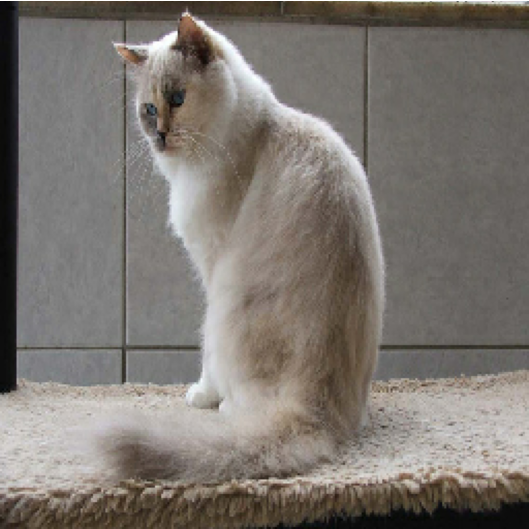
\includegraphics[width=1\linewidth]{recursos/imagens/project/pets_ori.png}
        \caption{Imagem original do animal de estimação.}
        \label{project:fig:dataset:pets_1.1}
    \end{subfigure}%
    ~ 
    \begin{subfigure}[t]{0.45\textwidth}
        \centering
        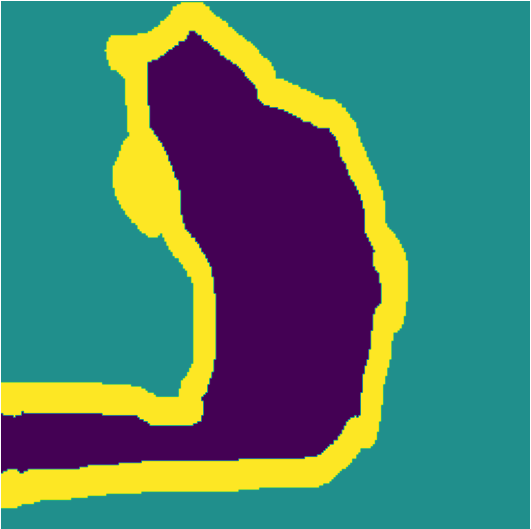
\includegraphics[width=1\linewidth]{recursos/imagens/project/pets_mask.png}
        \caption{Máscara com fundo em verde, contorno em amarelo e animal em roxo.}
        \label{project:fig:dataset:pets_1.2}
    \end{subfigure}%

    Fonte: retirado e adaptado de \cite{Parkhi2012CatsDogs}.
\end{figure}

Vale dizer que originalmente essas amostras estão separadas entre $3.669$ ($49,925\%$) para a etapa de teste e $3.680$ ($50,075\%$) para a etapa de treinamento. Todavia, nos testes realizados foi utilizado também um conjunto de dados voltado para validação, o qual foi extraído a partir do \textit{dataset} de teste, sendo assim, para o presente trabalho, a divisão passou a ser de $669$ exemplos para teste, 3.000 amostras para validação e 3.680 instâncias para treino, levando em conta os conceitos tratados na Seções \ref{deep:train} e \ref{deep:test}.

É relevante salientar que as imagens do conjunto de dados original são tridimensionais, ou seja, cada amostra inclui informações dos canais de cores vermelho, verde e azul. Já as máscaras são unidimensionais, apresentando um mapa de valores singulares para representar as regiões de interesse baseadas na imagem original. Os valores numéricos nas máscaras correspondem ao fundo, à borda ou ao animal.

Vale observar que diferentemente de muitos outros conjuntos de dados de imagem \citep{Bossard2014Food-101Forests}, o \textit{Oxford-III Pets} não apresenta dimensões padronizadas para suas amostras. Todavia, no atual trabalho, houve uma alteração nesse aspecto, em que foram aplicadas duas técnicas, além da técnica de aumento de dados que será discutida na Seção \ref{project:augment}, em todos os exemplos do conjunto de dados. Sendo que a primeira técnica aplicada foi a padronização tanto das imagens originais, quanto das máscaras, em relação às suas dimensões, em que ambas passaram a ter o valor de $256 \times 256$, que é o um valor comumente utilizado na área de imagens para substanciar as características da mesma \citep{Lee1983DigitalFilter}.

Além disso, procedeu-se à normalização dos valores do conjunto de dados. Tanto as imagens quanto as máscaras foram normalizadas para um intervalo de $0$ a $1$, como indicado pela Equação \ref{project:eq:dataset:pets_1}.

\begin{equation}
    \label{project:eq:dataset:pets_1}
    \text{imagem de entrada normalizada}_{(i,j,k)} = \frac{\text{imagem de entrada}_{(i,j,k)}}{255},
\end{equation}
onde $(i,j,k)$ representa as coordenadas de altura, largura e canal, respectivamente.

No caso das máscaras, essa normalização foi realizada subtraindo-se um valor unitário de cada pixel que inicialmente correspondia a 1, 2 e 3, representando o animal em questão, a borda e o fundo, respectivamente. Esse procedimento permitiu transformar o intervalo de valores para $0$ a $1$, conforme descrito pela Equação \ref{project:eq:dataset:pets_2}.

\begin{equation}
    \label{project:eq:dataset:pets_2}
    \text{máscara de entrada normalizada} = \text{máscara de entrada} - 1,
\end{equation}
em que, assim como na Equação \ref{project:eq:dataset:pets_1}, $(i,j,k)$ representa as coordenadas de altura, largura e canal, respectivamente.

Por fim, é relevante ressaltar que esse conjunto de dados se mostra adequado para o treinamento em segmentação semântica, uma vez que conta com todos os dados devidamente rotulados, proporcionando um cenário propício para esse propósito. O resultado gerado por essa abordagem será um mapa de características, ilustrado de forma análoga ao apresentado na Figura \ref{project:fig:dataset:pets_1.2}.

\paragraph{CIFAR 100}
\label{project:dataset:cifar}
O conjunto de dados CIFAR-100 \footnote{Conjuntos de dados CIFAR-10 e CIFAR-100 - \url{https://www.cs.toronto.edu/~kriz/cifar.html}} \citep{Krizhevsky2014TheDataset} é composto por um total de $60.000$ imagens, cada uma com dimensões de $32 \times 32$ pixels. Estas imagens são categorizadas em $20$ \quotes{superclasses}, cada uma contendo $5$ \quotes{classes finas}.

De maneira geral, o \textit{dataset} possui $100$ classes, com $600$ amostras em cada classe. Cada exemplo neste conjunto de dados é rotulado com uma \textit{superclass}, que representa uma categoria mais abrangente (como "veículo"), e uma \textit{fine class}, que representa uma categoria mais específica (como \quotes{bicicleta}, \quotes{ônibus}, etc.). Alguns exemplos dessas amostras podem ser visualizados na Figura \ref{project:fig:dataset:cifar}.

\begin{figure}[H]
    \centering
    \caption{Exemplos de amostras do conjunto de dados CIFAR-100.}
    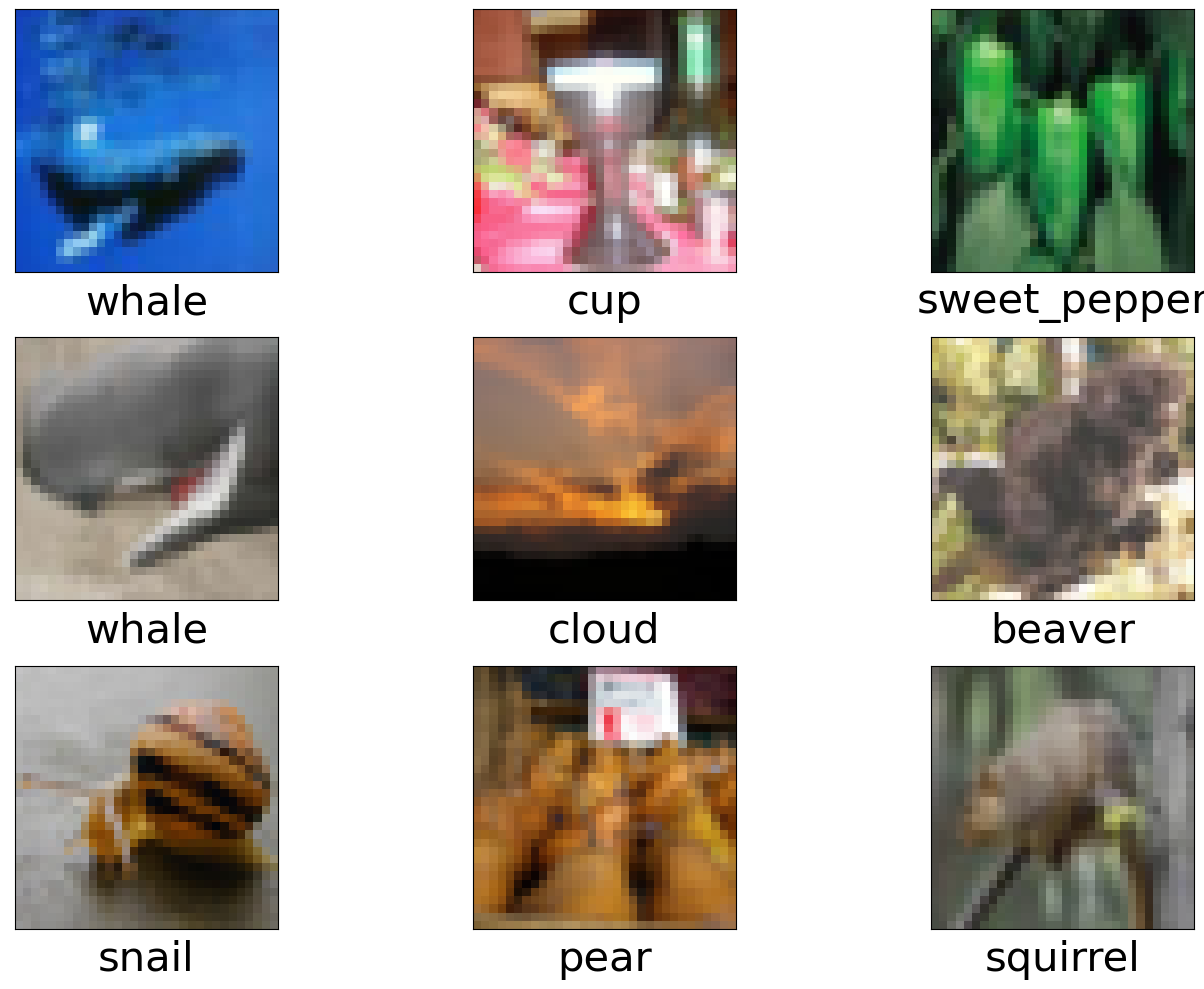
\includegraphics[width=1\textwidth]{recursos/imagens/project/cifar100v2.png}
    \label{project:fig:dataset:cifar}

    Fonte: retirado e adaptado de \cite{Krizhevsky2014TheDataset}.
\end{figure}

Em contraste com a configuração original proposta por \cite{Krizhevsky2014TheDataset}, dividimos o conjunto de dados em $83,33\%$ para treinamento, $11,66\%$ para validação e $5\%$ para teste, visando evitar qualquer viés nos resultados, conforme recomendado por \cite{Domingos2012ALearning}. Além de aplicar um processo de normalização das amostras, deixando o valor de todos os pixels das amostras entre o domínio de $[0, 1]$, com um processo muito semelhante ao da Equação \ref{project:eq:dataset:pets_1}.

Finalmente, vale citar que todas as imagens do conjunto de dados se encontram rotuladas e prontas para serem usadas na tarefa de classificação.

\paragraph{\textit{Food}-101}
\label{project:dataset:food101}
O conjunto de dados \textit{Food}-101 \footnote{Conjunto de dados \textit{Food}-101 - \url{https://data.vision.ee.ethz.ch/cvl/datasets_extra/food-101/}} \citep{Bossard2014Food-101Forests} foi empregado como um segundo conjunto de dados para a classificação de imagens neste trabalho. Este \textit{dataset} contém $101.000$ imagens, originalmente com uma resolução de $512 \times 512$ pixels, no entanto, para otimizar o processamento do modelo e manter a representatividade da amostra, essas imagens foram redimensionadas para $224 \times 224$ pixels.

Ao contrário do conjunto CIFAR-100, que abrange classes mais generalistas (vide Seção \ref{project:dataset:cifar}), o conjunto de dados \textit{Food}-101 se concentra exclusivamente em classes relacionadas à alimentação. Ele é composto por $101$ classes (por exemplo, \quotes{pizza}, \quotes{bruscheta}, entre outros), cada uma com $1.000$ amostras. Alguns exemplos dessas classes podem ser visualizados na Figura \ref{project:fig:dataset:food}.

\begin{figure}[H]
    \centering
    \caption{Exemplos de amostras do conjunto de dados \textit{Food}-101.}
    \label{project:fig:dataset:food}
    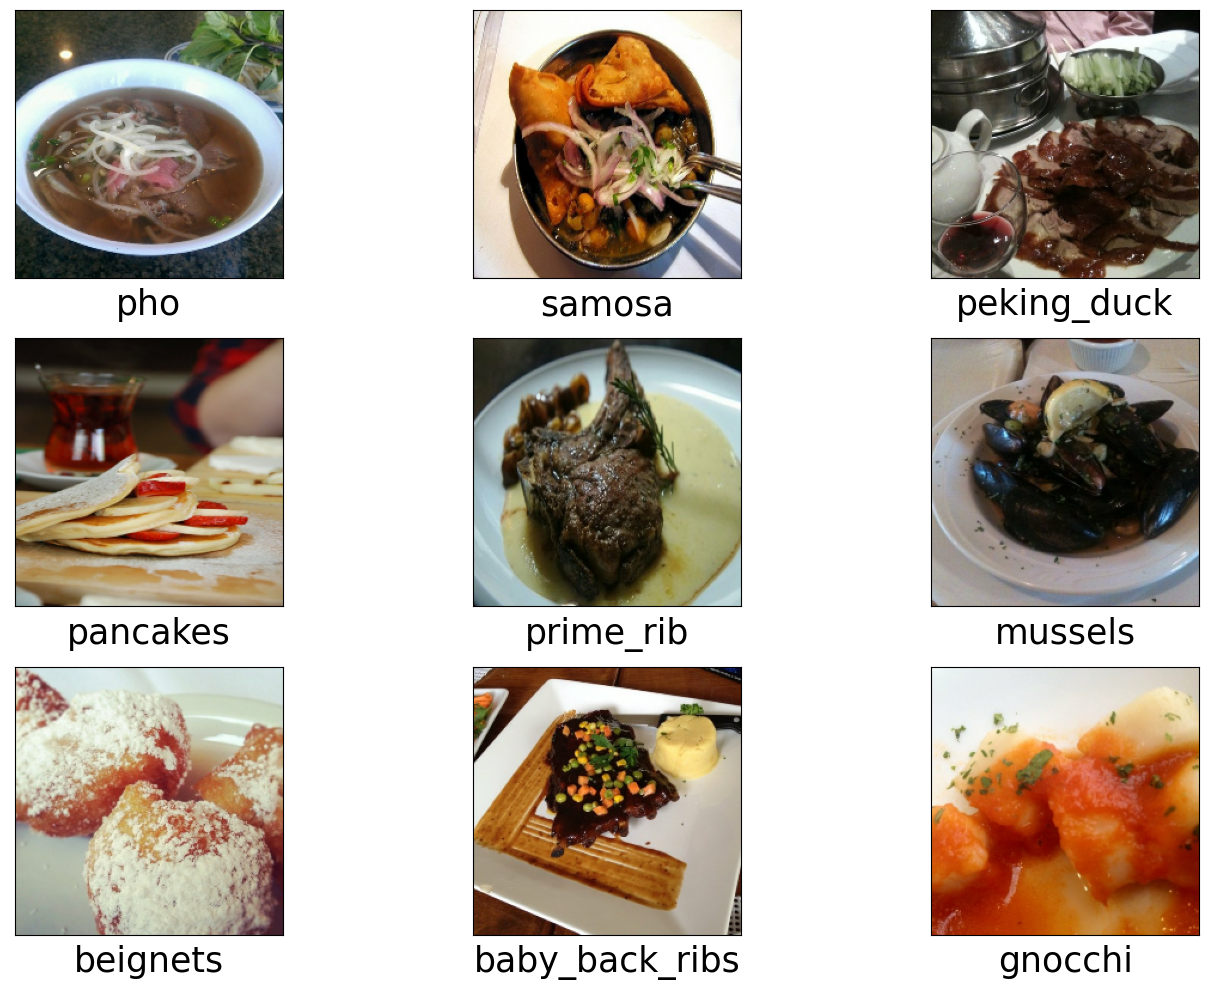
\includegraphics[width=1\textwidth]{recursos/imagens/project/food101v2.png}

    Fonte: Adaptado de \cite{Bossard2014Food-101Forests}.
\end{figure}

Adicionalmente, houve uma reorganização do conjunto de dados em relação à sua configuração original, sendo que $75\%$ das amostras foram designadas para o conjunto de treinamento, $17,5\%$ para validação e $7,5\%$ para teste. Além disso, foi aplicado um pré-processamento de normalização, conforme representado na Equação \ref{project:eq:dataset:pets_1}, com o intuito de reduzir o viés do modelo durante o treinamento \citep{Shorten2019ALearning}.

É importante ressaltar também que o conjunto de dados \textit{Food}-101 também foi empregado no processo de classificação de imagens. Ele atua como um conjunto alternativo, permitindo demonstrar a capacidade de generalização do modelo e da técnica utilizada em diversos cenários. Devido ao seu tamanho, uma amostra do \textit{dataset} \textit{Food}-101 contém aproximadamente dezesseis vezes mais informações do que uma amostra do CIFAR-100, o que proporciona uma maior riqueza de detalhes e complexidade para o treinamento e validação do modelo.

\subsubsection{Transferência de Aprendizado}
\label{project:transf}
A técnica de transferência de aprendizado, empregada neste estudo, encontra inspiração em cenários do cotidiano, onde um conhecimento prévio sobre um tema pode ser crucial para acelerar e incrementar a aprendizagem de novos conteúdos \citep{Pan2010}. Esta técnica mostra-se especialmente útil em situações onde se dispõe de um conjunto de dados alvo com uma quantidade limitada de amostras para o treinamento de uma rede \citep{Weiss2016}, considerando que Redes Profundas necessitam vastas quantidades de dados para obter um desempenho satisfatório \citep{Goodfellow2016}.

Sob essa perspectiva, o treinamento das redes de classificação VGG-16 para os conjuntos de dados CIFAR 100 e \textit{Food}-101 se ancorou nos conceitos de transferência de aprendizado. Utilizamos os pesos da rede VGG16 pré-treinada no \textit{dataset} ImageNet\footnote{Conjunto de dados ImageNet - \url{https://www.image-net.org/download.php}} \citep{Deng2009ImageNet:Database}, que dispõe de um milhar ($1.000$) de classes com $1.281.167$, $50.000$ e $100.000$ exemplos para treinamento, validação e testes, respectivamente.

Dessa forma, a inicialização da rede neural ocorreu com os pesos pré-treinados da VGG-16. Ao longo dos treinamentos, foi empregado o procedimento de descongelamento progressivo das camadas da VGG-16, começando pelas camadas densas e alcançando até o terceiro bloco convolucional, sem ultrapassar esse ponto para preservar as características de baixo nível presentes nos pesos do treinamento com o ImageNet. A estratégia adotada foi a de alternar entre o descongelamento de blocos e a continuação dos treinamentos, sempre escolhendo o melhor modelo, conforme exemplificado na Figura \ref{project:fig:transf1} e sugerido por \cite{Chollet2021DeepPython}. Essa abordagem foi aplicada em ambos os conjuntos de dados e nos métodos de \textit{pooling} avaliados (\textit{AvgPooling}, \textit{MaxPooling} e BPCAPooling).

\begin{figure}[H]
    \centering
    \caption{Processo de \textit{fine-tuning} da VGG-16, com o descongelamento dos blocos representados pelo fundo azul.}
    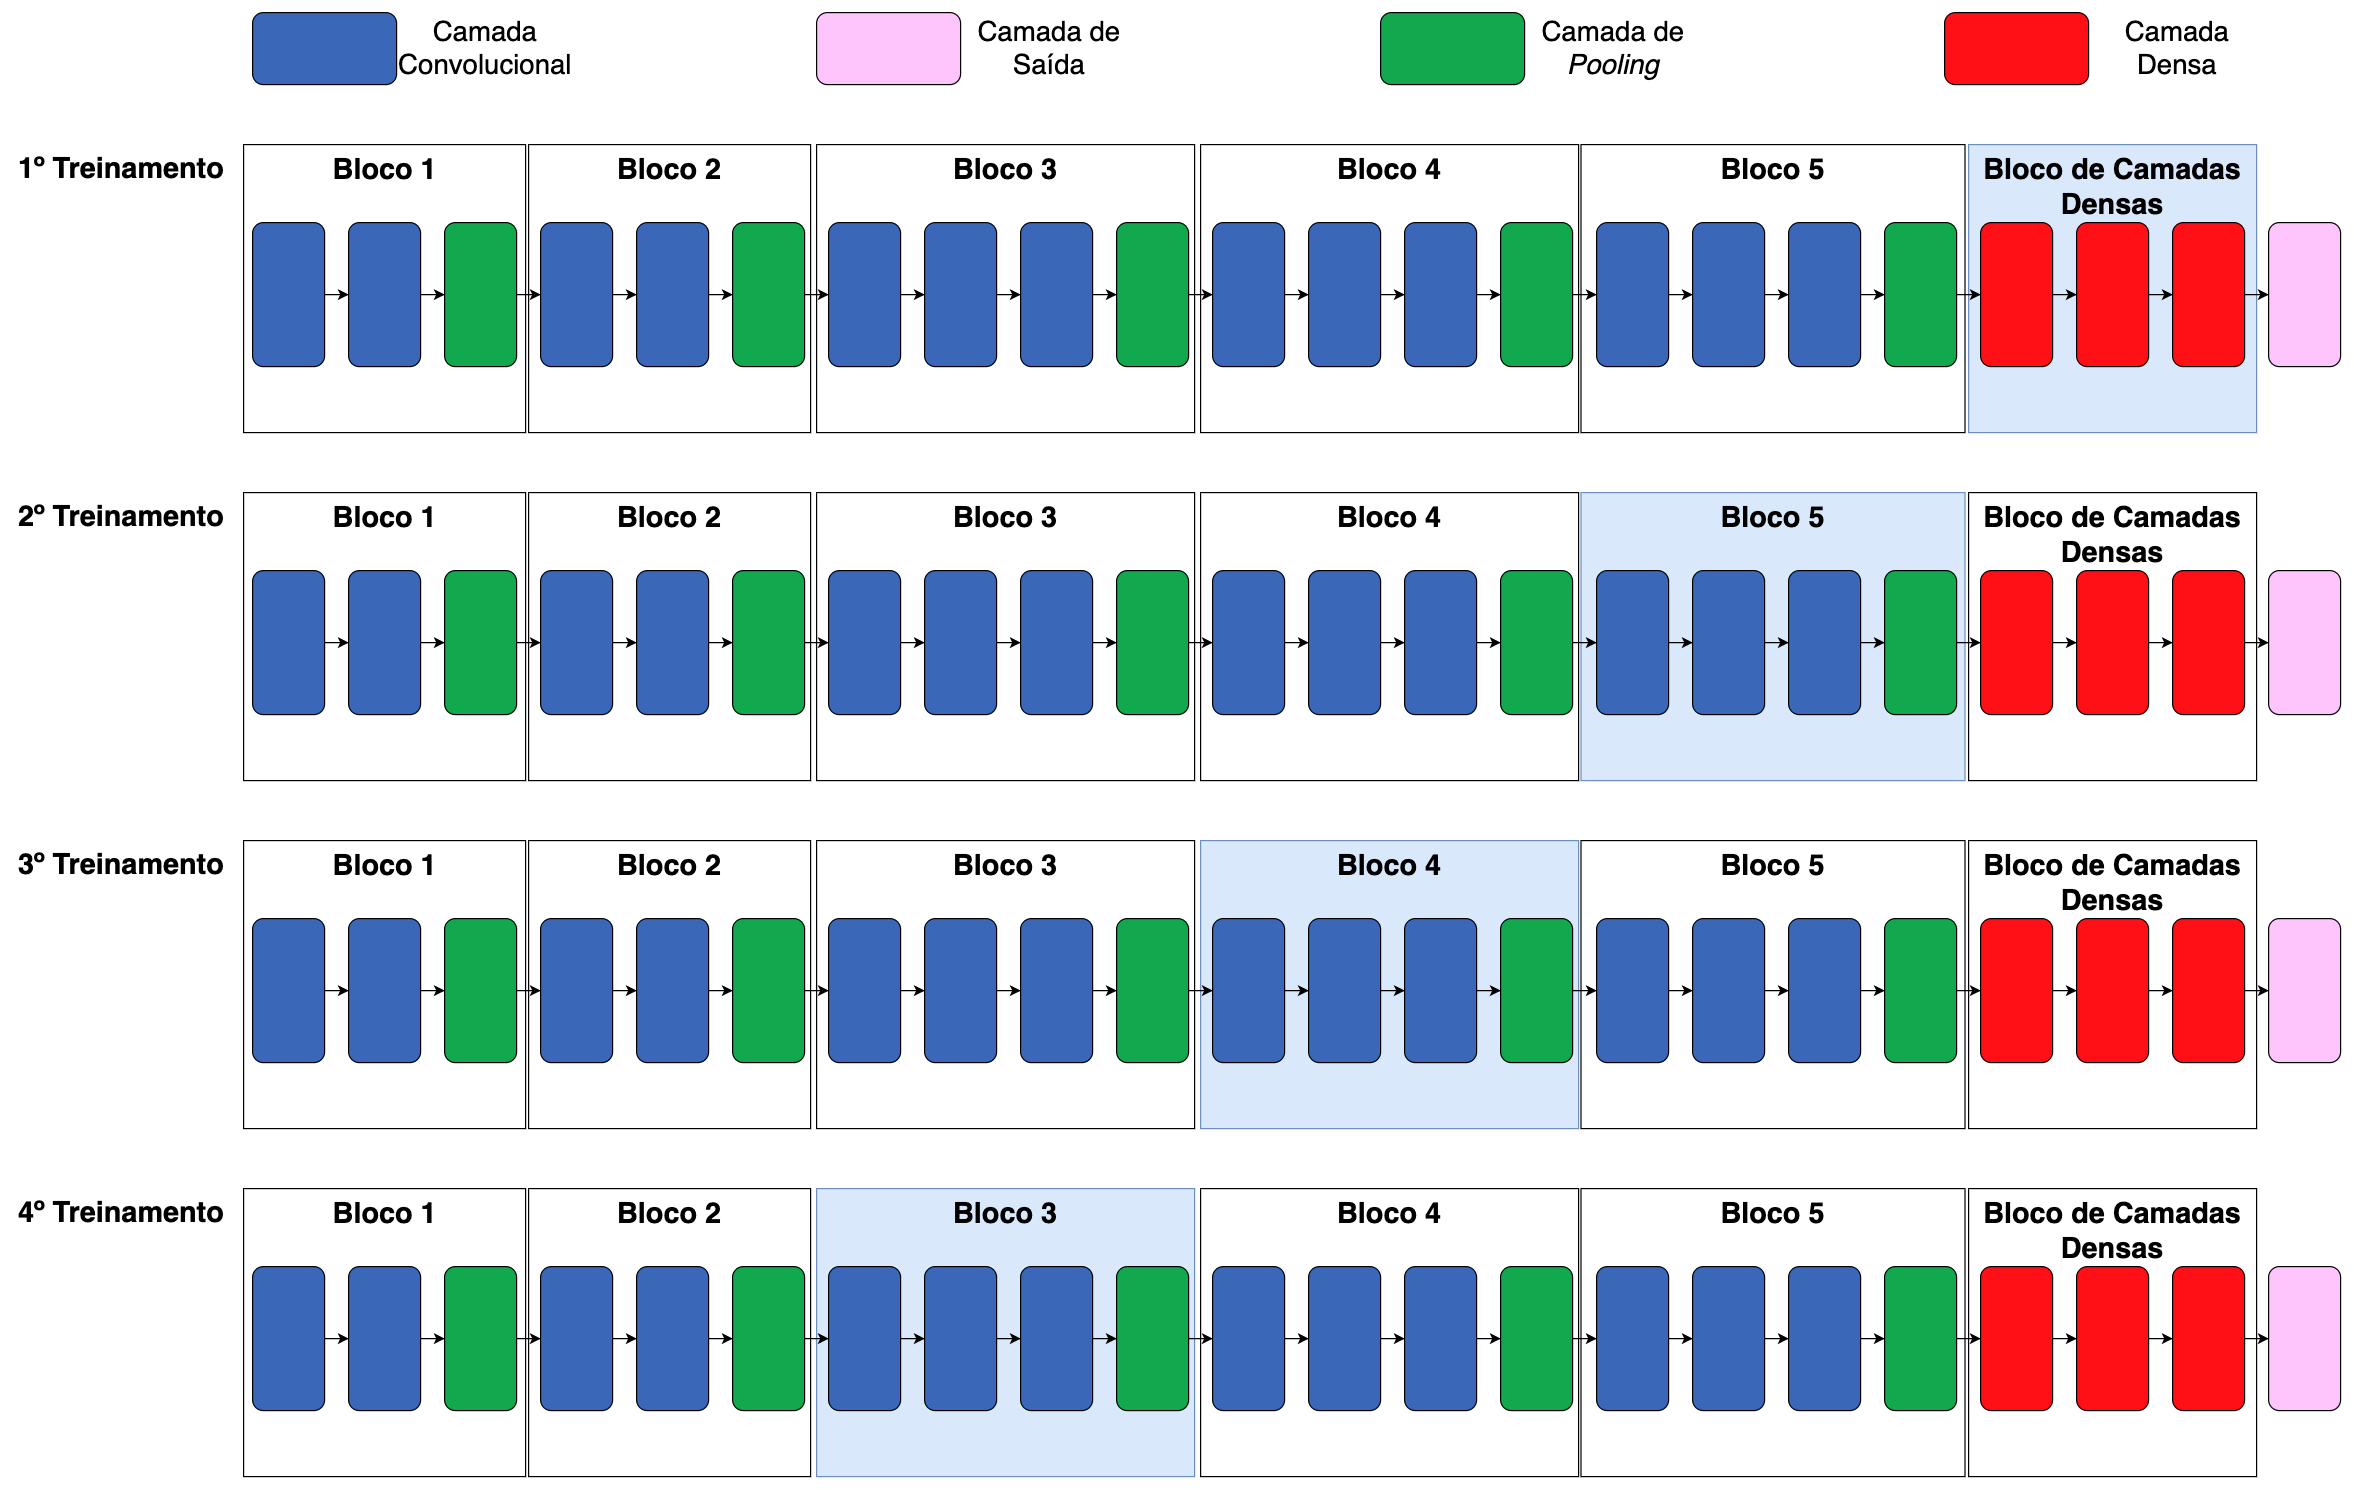
\includegraphics[width=1\textwidth]{recursos/imagens/project/fine-tunning.png}
    \label{project:fig:transf1}

    Fonte: do próprio autor.
\end{figure}

No que tange aos testes efetuados com os modelos U-Net e U-Net-Like, é relevante salientar que não se empregou as técnicas de transferência de aprendizado, devido a alguns aspectos cruciais da própria técnica. O primeiro desafio é a necessidade de utilizar a mesma arquitetura para o modelo de base adotado para a transferência de aprendizado e para o modelo treinado. Ainda que soluções para essa questão tenham sido propostas, como a adoção de camadas da VGG-16 dentro da estrutura de uma U-Net \citep{Pravitasari2020UNet-VGG16Segmentation}, a aplicação de tal técnica poderia afetar os resultados pretendidos decorrentes exclusivamente da modificação da camada de \textit{pooling} nos modelos U-Net e U-Net-Like. Adicionalmente, a escassez de conjuntos de dados robustos, similares ao ImageNet, direcionados ao processo de segmentação semântica, configura outro obstáculo, especialmente considerando a falta de padronização no formato das anotações. Como referência para um adequado conjunto de dados e modelo de anotação, podemos citar o COCO-\textit{stuff} \citep{Caesar2016} e o formato de anotação COCO, que pode ser desenvolvido a partir da ferramenta \textit{COCO Annotator} \citep{Brooks2019COCOAnnotator}.


\subsubsection{Aumento de Dados}
\label{project:augment}
O uso de técnicas de aumento de dados tem se revelado eficaz para o fortalecimento da capacidade de aprendizado dos modelos, especialmente no que tange à mitigação de problemas de \textit{overfitting}, como discutido na Seção \ref{cnn:augment}. Portanto, é relevante destacar a importância da implementação de transformações geométricas e de intensidade de cor, as quais foram empregadas de forma diversificada e com base em uma abordagem probabilística estocástica nos experimentos desenvolvidos neste trabalho. Adicionalmente, cabe enfatizar que a probabilidade de aplicação do aumento de dados durante o processo de treinamento a cada imagem pode resultar na aplicação simultânea de múltiplas transformações na mesma imagem.

É importante enfatizar que, em todos os conjuntos de dados utilizados, a técnica de aumento de dados foi aplicada exclusivamente nos subconjuntos de treinamento. Esta abordagem foi adotada considerando que os subconjuntos de teste e validação são empregados para avaliar o desempenho do modelo, não para ensiná-lo em diferentes cenários.

As próximas seções, especificamente \ref{project:augment:cifar}, \ref{project:augment:food}, e \ref{project:augment:pets}, discutem as transformações aplicadas nos conjuntos de dados CIFAR 100, \textit{Food}-101 e \textit{Oxford-IIIT Pets}, respectivamente. Estas discussões proporcionam \textit{insights} relevantes que poderão orientar futuras pesquisas na área e facilitar a reprodução dos testes conduzidos neste estudo.

\paragraph{CIFAR 100}
\label{project:augment:cifar}
Para o conjunto de dados CIFAR 100, optou-se primordialmente por aplicar transformações geométricas como técnicas de aumento de dados. Considerando a diversidade das classes presentes no conjunto e o baixo risco de distorção de significado do rótulo do exemplo em questão - uma preocupação discutida por \cite{Shorten2019ALearning} no contexto do conjunto de dados MNIST -, foi possível utilizar transformações com uma variação considerável sem, contudo, deixar a imagem irreconhecível para a interpretação humana.

As transformações aplicadas no conjunto de dados CIFAR 100, bem como a variação permitida para cada uma delas, estão detalhadamente descritas na Tabela \ref{project:tab:augment:cifar}.

\begin{table}[H]
    \centering
    \caption{Transformações geométricas aplicadas no conjunto de dados CIFAR 100.}
    \label{project:tab:augment:cifar}
    \resizebox{0.6\textwidth}{!}{
    \begin{tabular}{l|l|l}
        \textbf{Tipo de transformação}              &  \textbf{Intervalo}        & \textbf{Parâmetro} \\ \hline
        Deslocamento Vertical                       &  $-25\% - 25\%$            &  -                 \\
        Deslocamento Horizontal                     &  $-25\% - 25\%$            &  -                 \\
        Cisalhamento                                &  $0^{\circ} - 25^{\circ}$  &  -                 \\
        \textit{Zoom}                               &  $0\% - 25\%$              &  -                 \\
        Rotação                                     &  $0^{\circ} - 45^{\circ}$  &  -                 \\
        Espelhamento Horizontal                     &  -                         &  Verdadeiro        \\
        Modo de Preenchimento                       &  -                         &  Mais próximo
    \end{tabular}}

    \vspace*{1 cm}
    Fonte: do próprio autor.
\end{table}

É importante ressaltar que, no contexto dos parâmetros listados na Tabela \ref{project:tab:augment:cifar}, os termos \quotes{Espelhamento Horizontal} e \quotes{Modo de Preenchimento} indicam, respectivamente, que a imagem pode ser submetida a um espelhamento horizontal e que o tipo de preenchimento escolhido, dentre as opções \quotes{constante}, \quotes{mais próximo}, \quotes{refletir} ou \quotes{envolver}, foi o método \quotes{mais próximo}. O efeito dessas transformações pode ser observado por meio do exemplo apresentado na Figura \ref{cnn:fig:augment}.

\paragraph{\textit{Food}-101}
\label{project:augment:food}
No que se refere ao \textit{dataset} \textit{Food}-101, é importante salientar que, apesar da técnica de aumento de dados ter sido aplicada e utilizada em alguns testes, somente foi possível implementá-la manualmente dentro do modelo. Isso resultou no aumento da complexidade do modelo padrão VGG-16, devido à necessidade de se acrescentar uma camada inicial responsável pela aplicação dos filtros de forma estocástica. Logo, os resultados comentados na Seção \ref{results}, referentes ao conjunto de dados \textit{Food}-101, não contemplam a aplicação da técnica de aumento de dados.

Ressalta-se, no entanto, que similarmente ao conjunto CIFAR 100, o \textit{dataset} \textit{Food}-101 não apresenta problemas relacionados à alteração da interpretação dos rótulos em função da aplicação do aumento de dados. Dessa forma, as transformações utilizadas para os testes são descritos na seguinte Tabela \ref{project:tab:augment:food}.

\begin{table}[H]
    \centering
    \caption{Transformações geométricas aplicadas no conjunto de dados \textit{Food}-101.}
    \label{project:tab:augment:food}
    \resizebox{0.6\textwidth}{!}{
    \begin{tabular}{l|l|l}
        \textbf{Tipo de transformação}              &  \textbf{Intervalo}         & \textbf{Parâmetro} \\ \hline
        Deslocamento Vertical                       &  $-25\% - 25\%$             &  -                 \\
        Deslocamento Horizontal                     &  $-25\% - 25\%$             &  -                 \\
        \textit{Zoom}                               &  $0\% - 25\%$               &  -                 \\
        Rotação                                     &  $-45^{\circ} - 45^{\circ}$ &  -                 \\
        Espelhamento Horizontal                     &  -                          &  Verdadeiro
    \end{tabular}}

    \vspace*{1 cm}
    Fonte: do próprio autor.
\end{table}

Neste conjunto de dados, nota-se uma ampliação na taxa de zoom em relação ao CIFAR, o que pôde ser explorado devido à maior resolução das amostras em relação ao primeiro conjunto. A representação visual do resultado da aplicação deste aumento de dados está evidenciada na Figura \ref{project:fig:augment:food}.

\begin{figure}[H]
   \centering
   \caption{Ilustração do aumento de dados com transformações geométricas aplicadas ao conjunto de dados \textit{Food}-101.}
   \label{project:fig:augment:food}
    \begin{subfigure}[t]{0.45\textwidth}
        \centering
        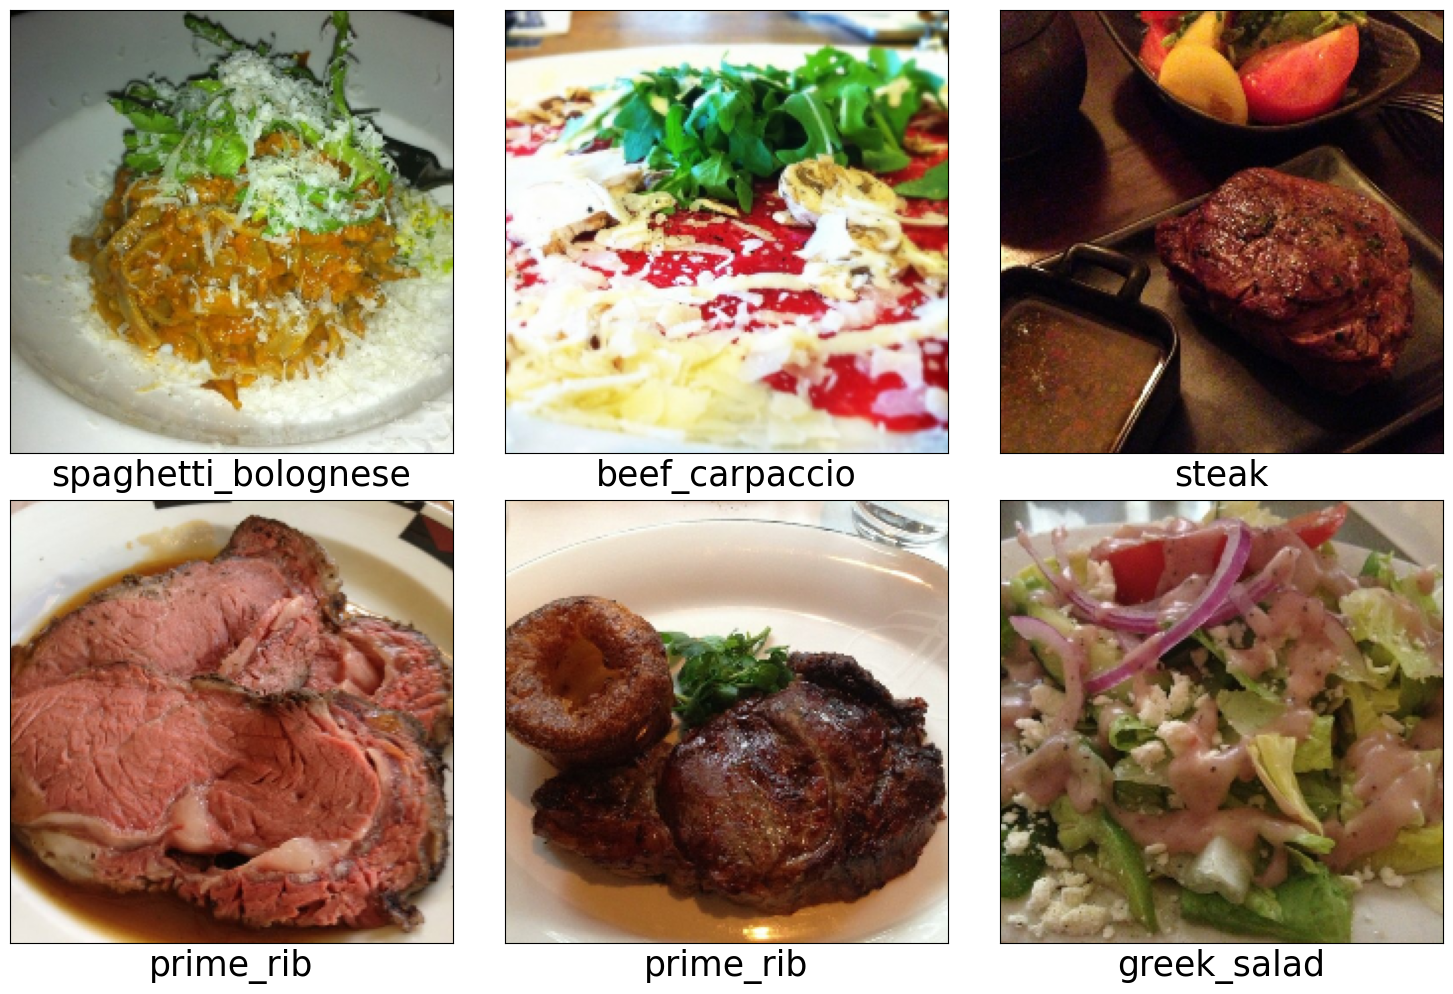
\includegraphics[width=1\linewidth]{recursos/imagens/project/dataaugmentation_o_food.png}
        \caption{Imagens Originais.}
        \label{project:fig:augment:food1.1}
    \end{subfigure}%
    ~ 
    \begin{subfigure}[t]{0.45\textwidth}
        \centering
        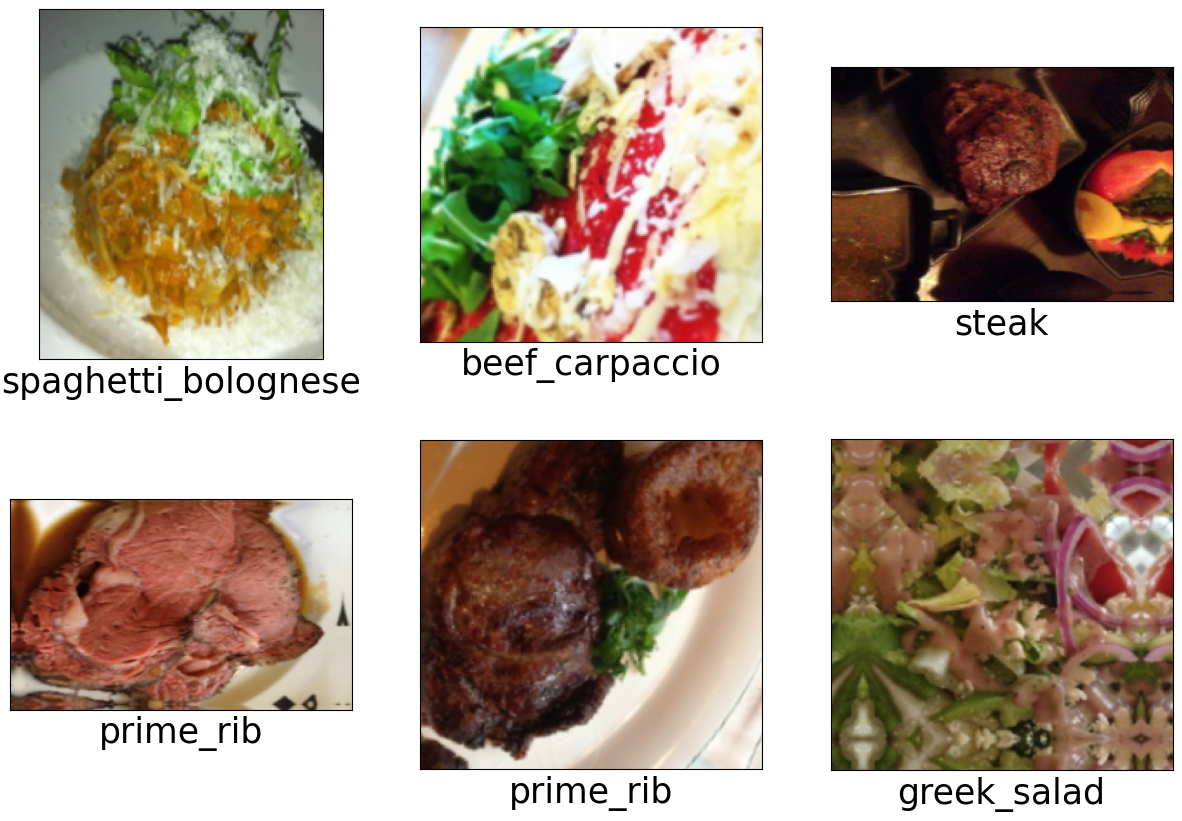
\includegraphics[width=1\linewidth]{recursos/imagens/project/dataaugmentation_food.png}
        \caption{Imagens com transformações.}
        \label{project:fig:augment:food1.2}
    \end{subfigure}%

    Fonte: do próprio autor. com base no conjunto de dados \textit{Food}-101 \citep{Bossard2014Food-101Forests}.
\end{figure}


\paragraph{\textit{Oxford-IIIT Pets}}
\label{project:augment:pets}
Para o conjunto de dados \textit{Oxford-IIIT Pets}, destinado à aplicação dos métodos de segmentação semântica com uso das arquiteturas U-Net-Like e convencionais U-Nets, um procedimento de aumento de dados foi implementado previamente à fase de treinamento dos modelos. Isto permitiu que as transformações empregadas fomentassem o aprendizado dos modelos e contribuíssem para a melhoria nas métricas de avaliação, que serão discutidas em detalhes na Seção \ref{project:exp_result}.

Contrariamente aos conjuntos de dados direcionados à classificação, nesse conjunto de dados foram aplicadas transformações que alteraram a cor das imagens, além de modificações geométricas. As especificações dessas transformações podem ser visualizadas na Tabela \ref{project:tab:augment:pets}.

\begin{table}[H]
    \centering
    \caption{Transformações executadas no conjunto de dados \textit{Oxford-IIIT Pets}.}
    \label{project:tab:augment:pets}
    \resizebox{0.6\textwidth}{!}{
    \begin{tabular}{l|l|l}
        \textbf{Tipo de transformação}              &  \textbf{Intervalo}         & \textbf{Parâmetro} \\ \hline
        Contraste                                   &  $0\% - 20\%$               &  -                 \\
        Brilho                                      &  $0\% - 35\%$               &  -                 \\
        Saturação                                   &  $0\% - 20\%$               &  -                 \\
        Rotação                                     &  $0^{\circ} - 90^{\circ}$   &  -                 \\
        Borramento                                  &  -                          &  Verdadeiro        \\
        Espelhamento Horizontal                     &  -                          &  Verdadeiro        \\
        Espelhamento Vertical                       &  -                          &  Verdadeiro
    \end{tabular}}

    \vspace*{1 cm}
    Fonte: do próprio autor.
\end{table}

Neste conjunto de dados, percebe-se que as transformações aplicadas são similares às aplicadas nos outros conjuntos de dados senão pelas transformações de cor. Entretanto, aqui os intervalos se referem às intensidades de alteração no contraste, brilho e saturação das imagens. A Figura \ref{project:fig:augment:pets} ilustra a aplicação aleatória das transformações descritas na Tabela \ref{project:tab:augment:pets}, juntamente com a máscara correspondente.

\begin{figure}[H]
    \centering
    \caption{Ilustração do aumento de dados com transformações aplicadas ao conjunto de dados \textit{Oxford-IIIT Pets}.}
    \label{project:fig:augment:pets}
    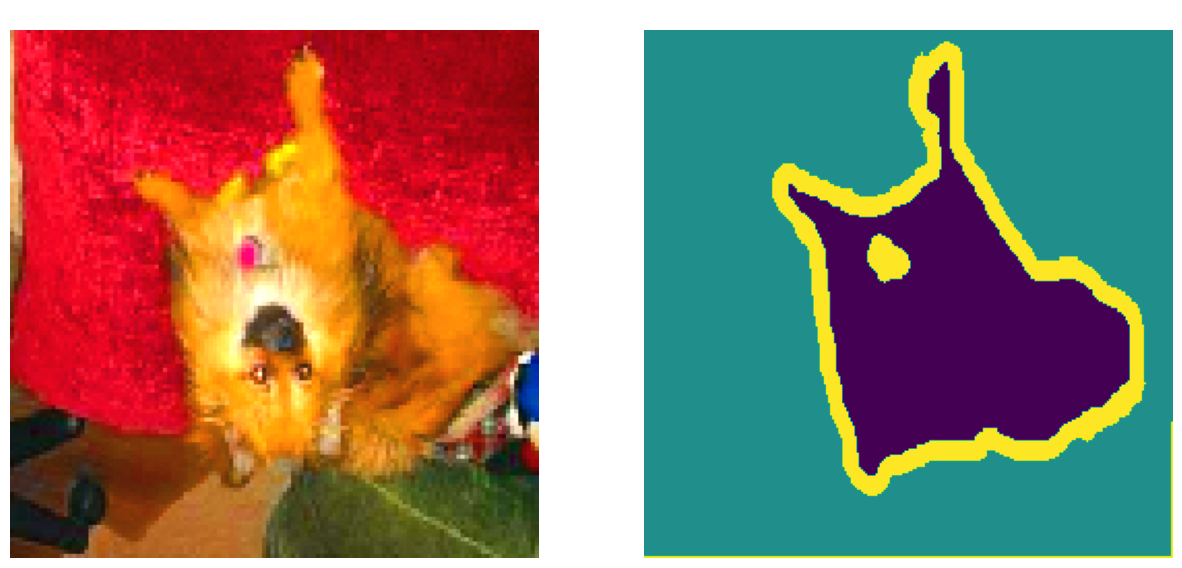
\includegraphics[width=1\textwidth]{recursos/imagens/project/dataaugmentation_pets.png}

    Fonte: do próprio autor. com base no conjunto de dados \textit{Oxford-IIIT Pets} \citep{Parkhi2012CatsDogs}.
\end{figure}

% Estas manipulações através do aumento de dados favorecem a robustez dos modelos empregados, potencializando a captura de características úteis e reduzindo a probabilidade de \textit{overfitting}, mesmo quando enfrentamos cenários com diversidade e quantidade insatisfatória de amostras.

\subsubsection{Alteração na Camada de \textit{Pooling}}
\label{project:change_pooling}
A camada de \textit{pooling} desempenha um papel crucial na arquitetura das CNNs, contribuindo significativamente para a redução da dimensionalidade e a invariância de translação, como mencionado na Seção \ref{cnn:pooling}. Nessa seção será discutido sobre a substituição das operações \textit{Max Pooling} e \textit{Average Pooling}, amplamente utilizadas \citep{Ozdemir2023Avg-topk:Networks}, nas arquiteturas VGG-16, U-Net-\textit{Like} e U-Net pelo método BPCAPooling que foi proposto no presente trabalho e é detalhado na Seção \ref{project:bpca}.

É fundamental salientar que a modificação da camada de \textit{pooling} envolveu a inclusão de argumentos adicionais para a camada. Enquanto os métodos de \textit{pooling} convencionais normalmente recebem parâmetros como a camada anterior, tamanho de passo (\textit{stride}) e tamanho da \textit{kernel}, para o processo BPCAPooling, além desses parâmetros, foi necessário especificar o número de componentes principais atribuídos a cada bloco. Tipicamente, esse número foi definido como $1$ para manter a consistência entre os tamanhos de blocos e o subconjunto de pixels (conforme discutido na Seção \ref{project:bpca}), e o tamanho esperado da saída, o que estava diretamente relacionado à quantidade de dados de entrada.

Na arquitetura VGG-16, utilizada para classificação de imagens nos conjuntos de dados CIFAR-100 e \textit{Food}-101, as camadas de \textit{Max Pooling} e \textit{Avg Pooling} foram substituídas pelo BPCAPooling. A Figura \ref{project:fig:change_pooling:vgg-cifar} ilustra essa substituição para o conjunto de dados CIFAR-100.

\begin{figure}[H]
    \centering
    \caption{Demonstração da substituição das camadas de \textit{pooling} convencionais por BPCAPooling no conjunto de dados CIFAR-100.}
    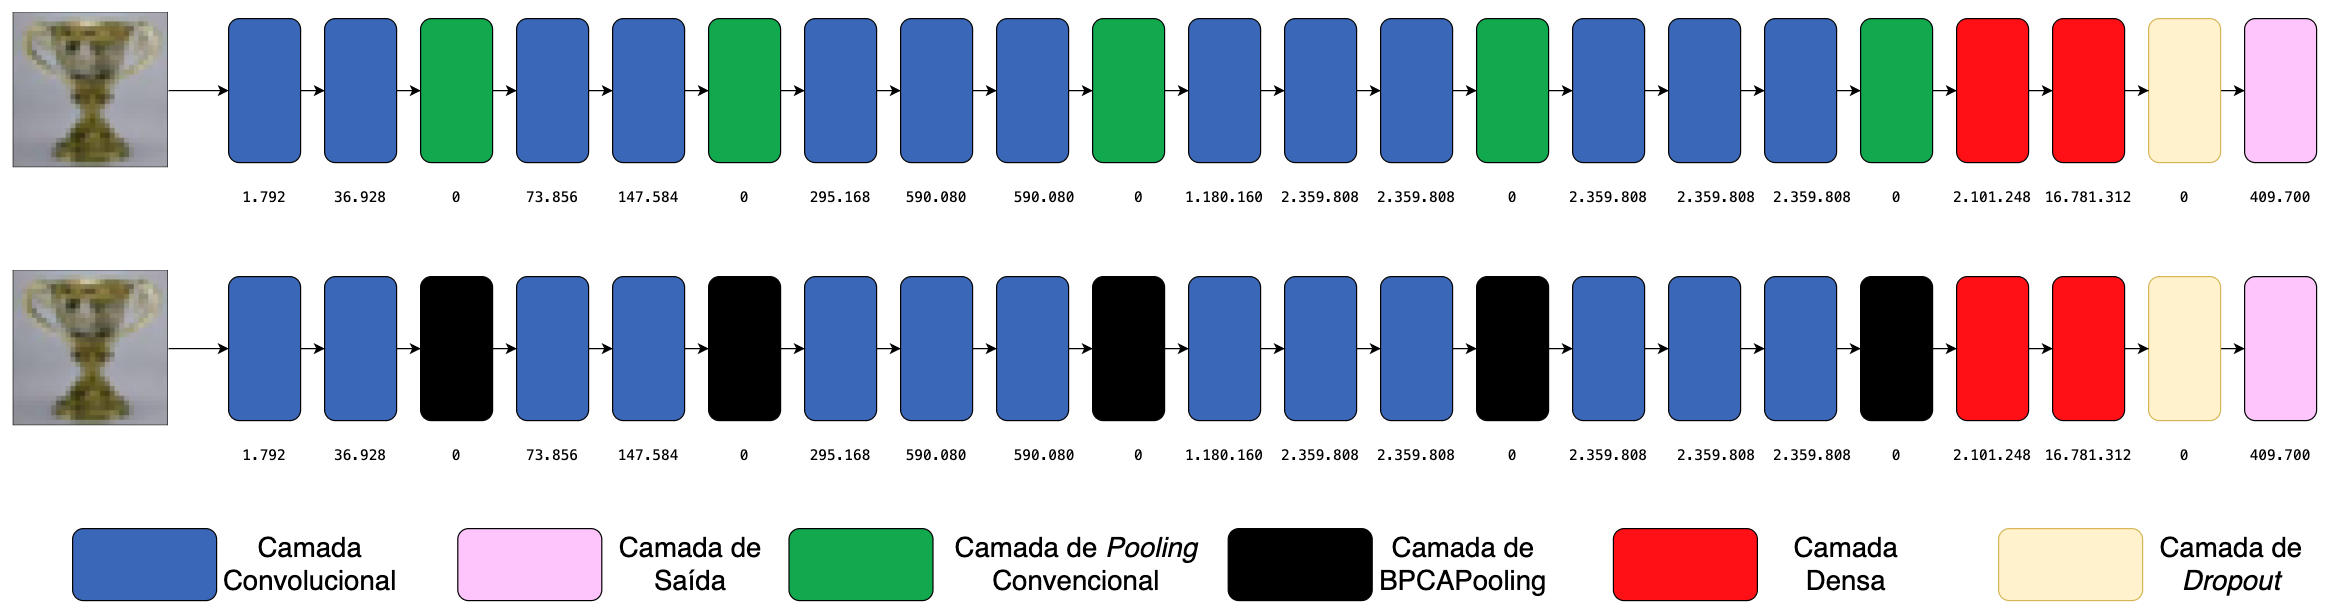
\includegraphics[width=1\textwidth]{recursos/imagens/project/vgg-with-bpca-cifar.png}
    \label{project:fig:change_pooling:vgg-cifar}

    Fonte: do próprio autor.
\end{figure}

Quanto à alteração da camada de \textit{pooling} na VGG-16 para o conjunto de dados \textit{Food}-101, a única diferença notável foi na camada de saída, que agora possui $413.797$ parâmetros. Isso se deve ao fato de que a camada de saída é sensível ao tamanho da imagem. A Figura \ref{project:fig:change_pooling:vgg-food} ilustra essa mudança para o conjunto de dados \textit{Food}-101.

\begin{figure}[H]
    \centering
    \caption{Demonstração da substituição das camadas de \textit{pooling} convencionais por BPCAPooling no conjunto de dados \textit{Food}-101.}
    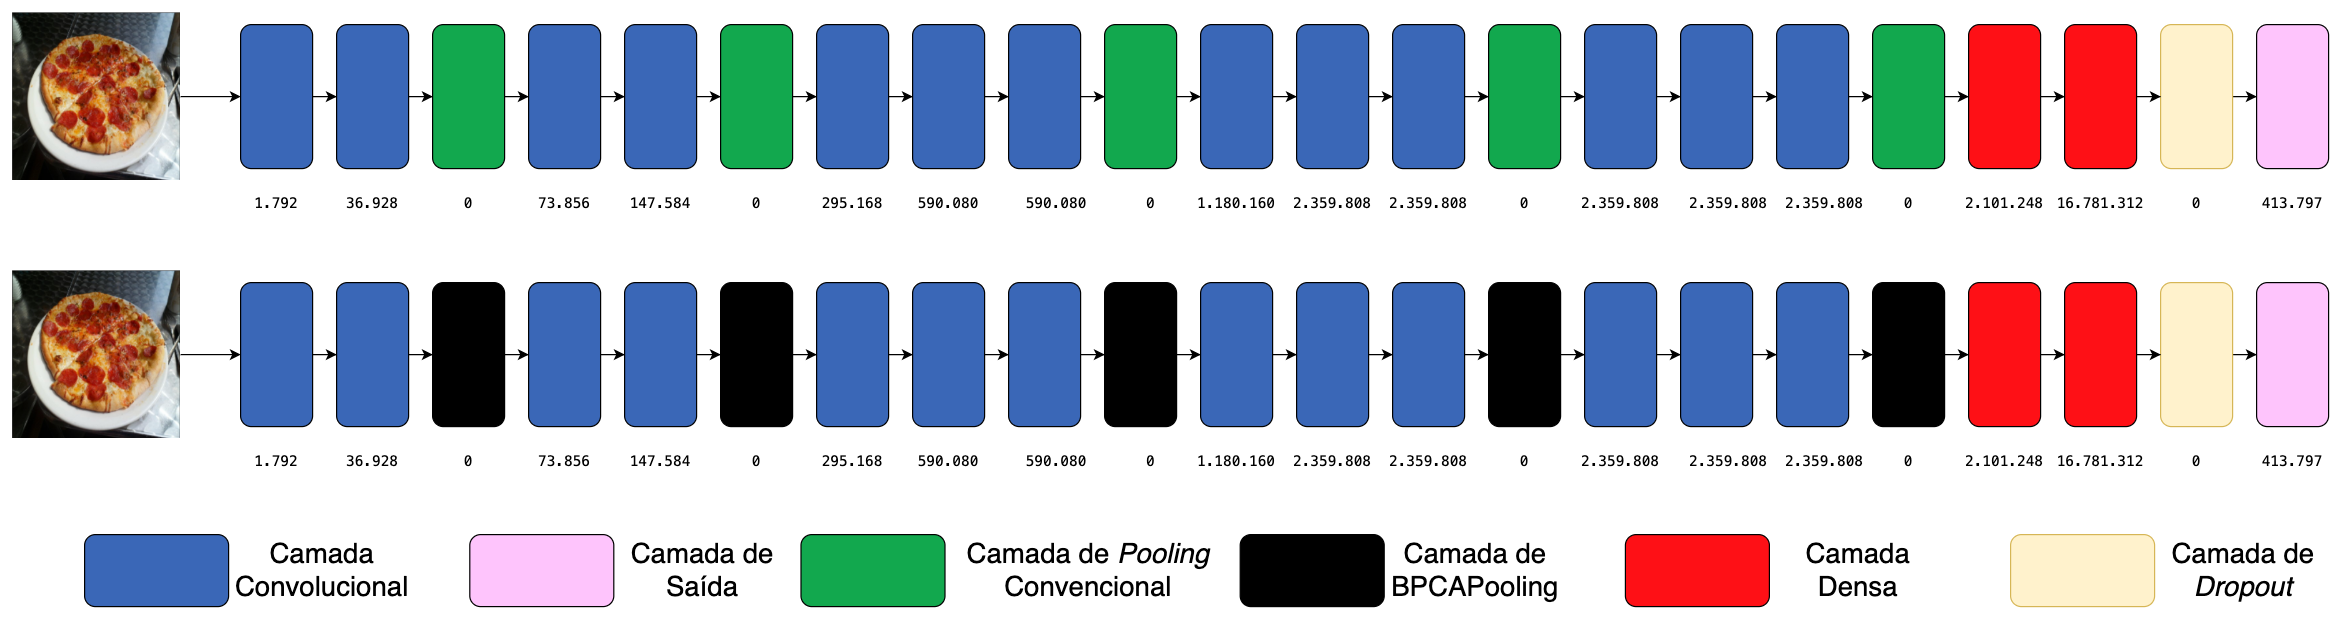
\includegraphics[width=1\textwidth]{recursos/imagens/project/vgg-with-bpca-food.png}
    \label{project:fig:change_pooling:vgg-food}

    Fonte: do próprio autor.
\end{figure}

Dessa forma, ao comparar as alterações nas camadas em relação à VGG-16 original para ambos os conjuntos de dados, nota-se a inclusão de uma camada de \textit{dropout} no final da rede, visando mitigar problemas de \textit{overfitting}, conforme discutido na Seção \ref{cnn:dropout}, que assim como as camadas de \textit{pooling}, não é visível uma influência quanto à quantidade de parâmetros treináveis. A rede para o conjunto de \textit{Food}-101 possui um total de $34.011.045$ de parâmetros, enquanto para o conjunto CIFAR-100, são $34.006.948$ parâmetros.

Da mesma forma, na arquitetura U-Net-\textit{Like}, empregada para segmentação semântica no conjunto de dados \textit{Oxford-IIIT Pets}, as camadas de \textit{Max Pooling} foram substituídas pela BPCAPooling. Vale ressaltar que, para as arquiteturas de segmentação semântica, não foi explorado o uso de \textit{Avg Pooling}, pois esse tipo de \textit{pooling} não é comumente empregado em arquiteturas de estado da arte \citep{Ronneberger2015U-net:Segmentation,Kugelman2022ASegmentation}. Essa adaptação foi realizada com o intuito de aprimorar a precisão da segmentação semântica, mantendo a informação espacial das entradas durante o processamento pelas diversas camadas. A ideia é que a estrutura geral da imagem fosse preservada ao longo das operações realizadas, garantindo que a imagem não fosse distorcida.

A arquitetura com as modificações citadas, bem como a quantidade de parâmetros treináveis ao lado da camada representada, pode ser visualizado na Figura \ref{project:fig:change_pooling:unet-like}.

\begin{figure}[H]
    \centering
    \caption{Arquitetura U-Net-\textit{Like} com aplicação de BPCAPooling.}
    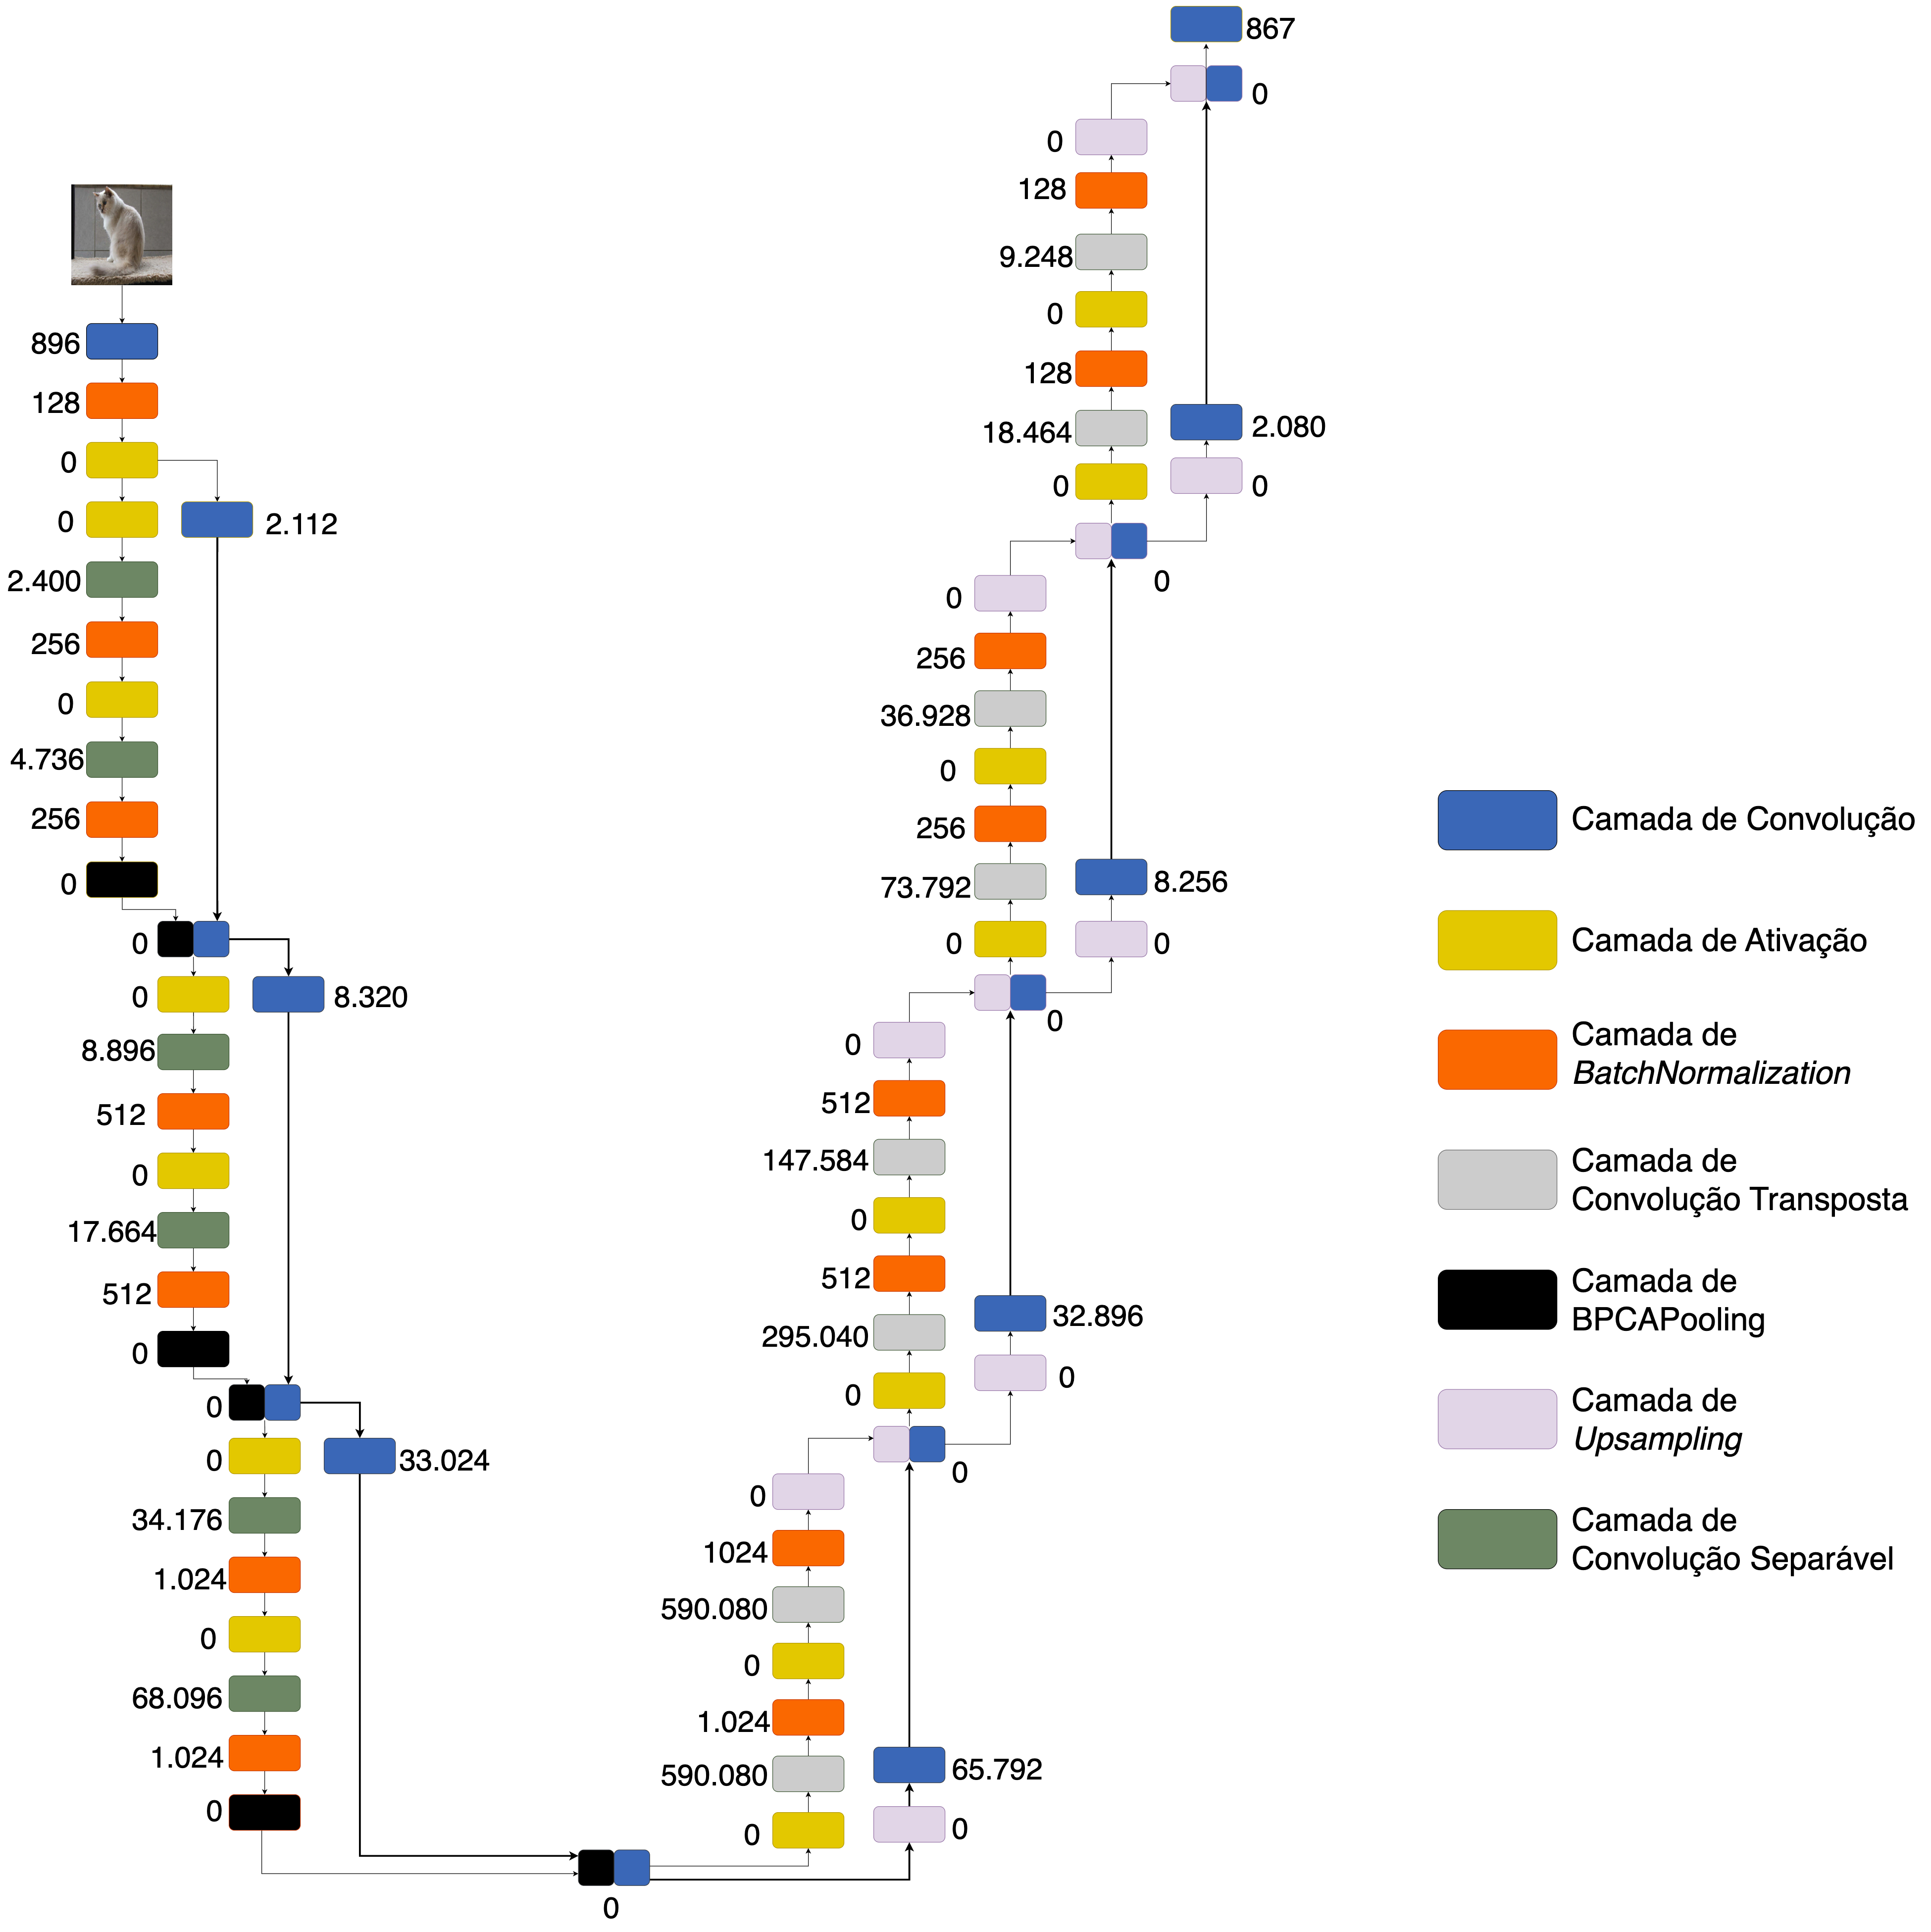
\includegraphics[width=1\textwidth]{recursos/imagens/project/unet-like-with-bpca-food.png}
    \label{project:fig:change_pooling:unet-like}

    Fonte: do próprio autor.
\end{figure}

Na arquitetura U-Net, também empregada para segmentação semântica, as camadas de \textit{Max Pooling} foram substituídas pelas camadas de BPCAPooling. Essa modificação busca aprimorar as capacidades de segmentação da arquitetura U-Net, proporcionando os mesmos benefícios descritos para a U-Net-\textit{Like}, porém de maneira mais robusta. A representação dessa adaptação está na Figura \ref{project:fig:change_pooling:unet}, similar às representações anteriores (\ref{project:fig:change_pooling:vgg-cifar} e \ref{project:fig:change_pooling:vgg-food}). Nessa figura, foi apresentada a arquitetura final com a aplicação do BPCAPooling, demonstrando a quantidade de parâmetros em cada camada.

\begin{figure}[H]
    \centering
    \caption{Arquitetura U-Net com aplicação de BPCAPooling.}
    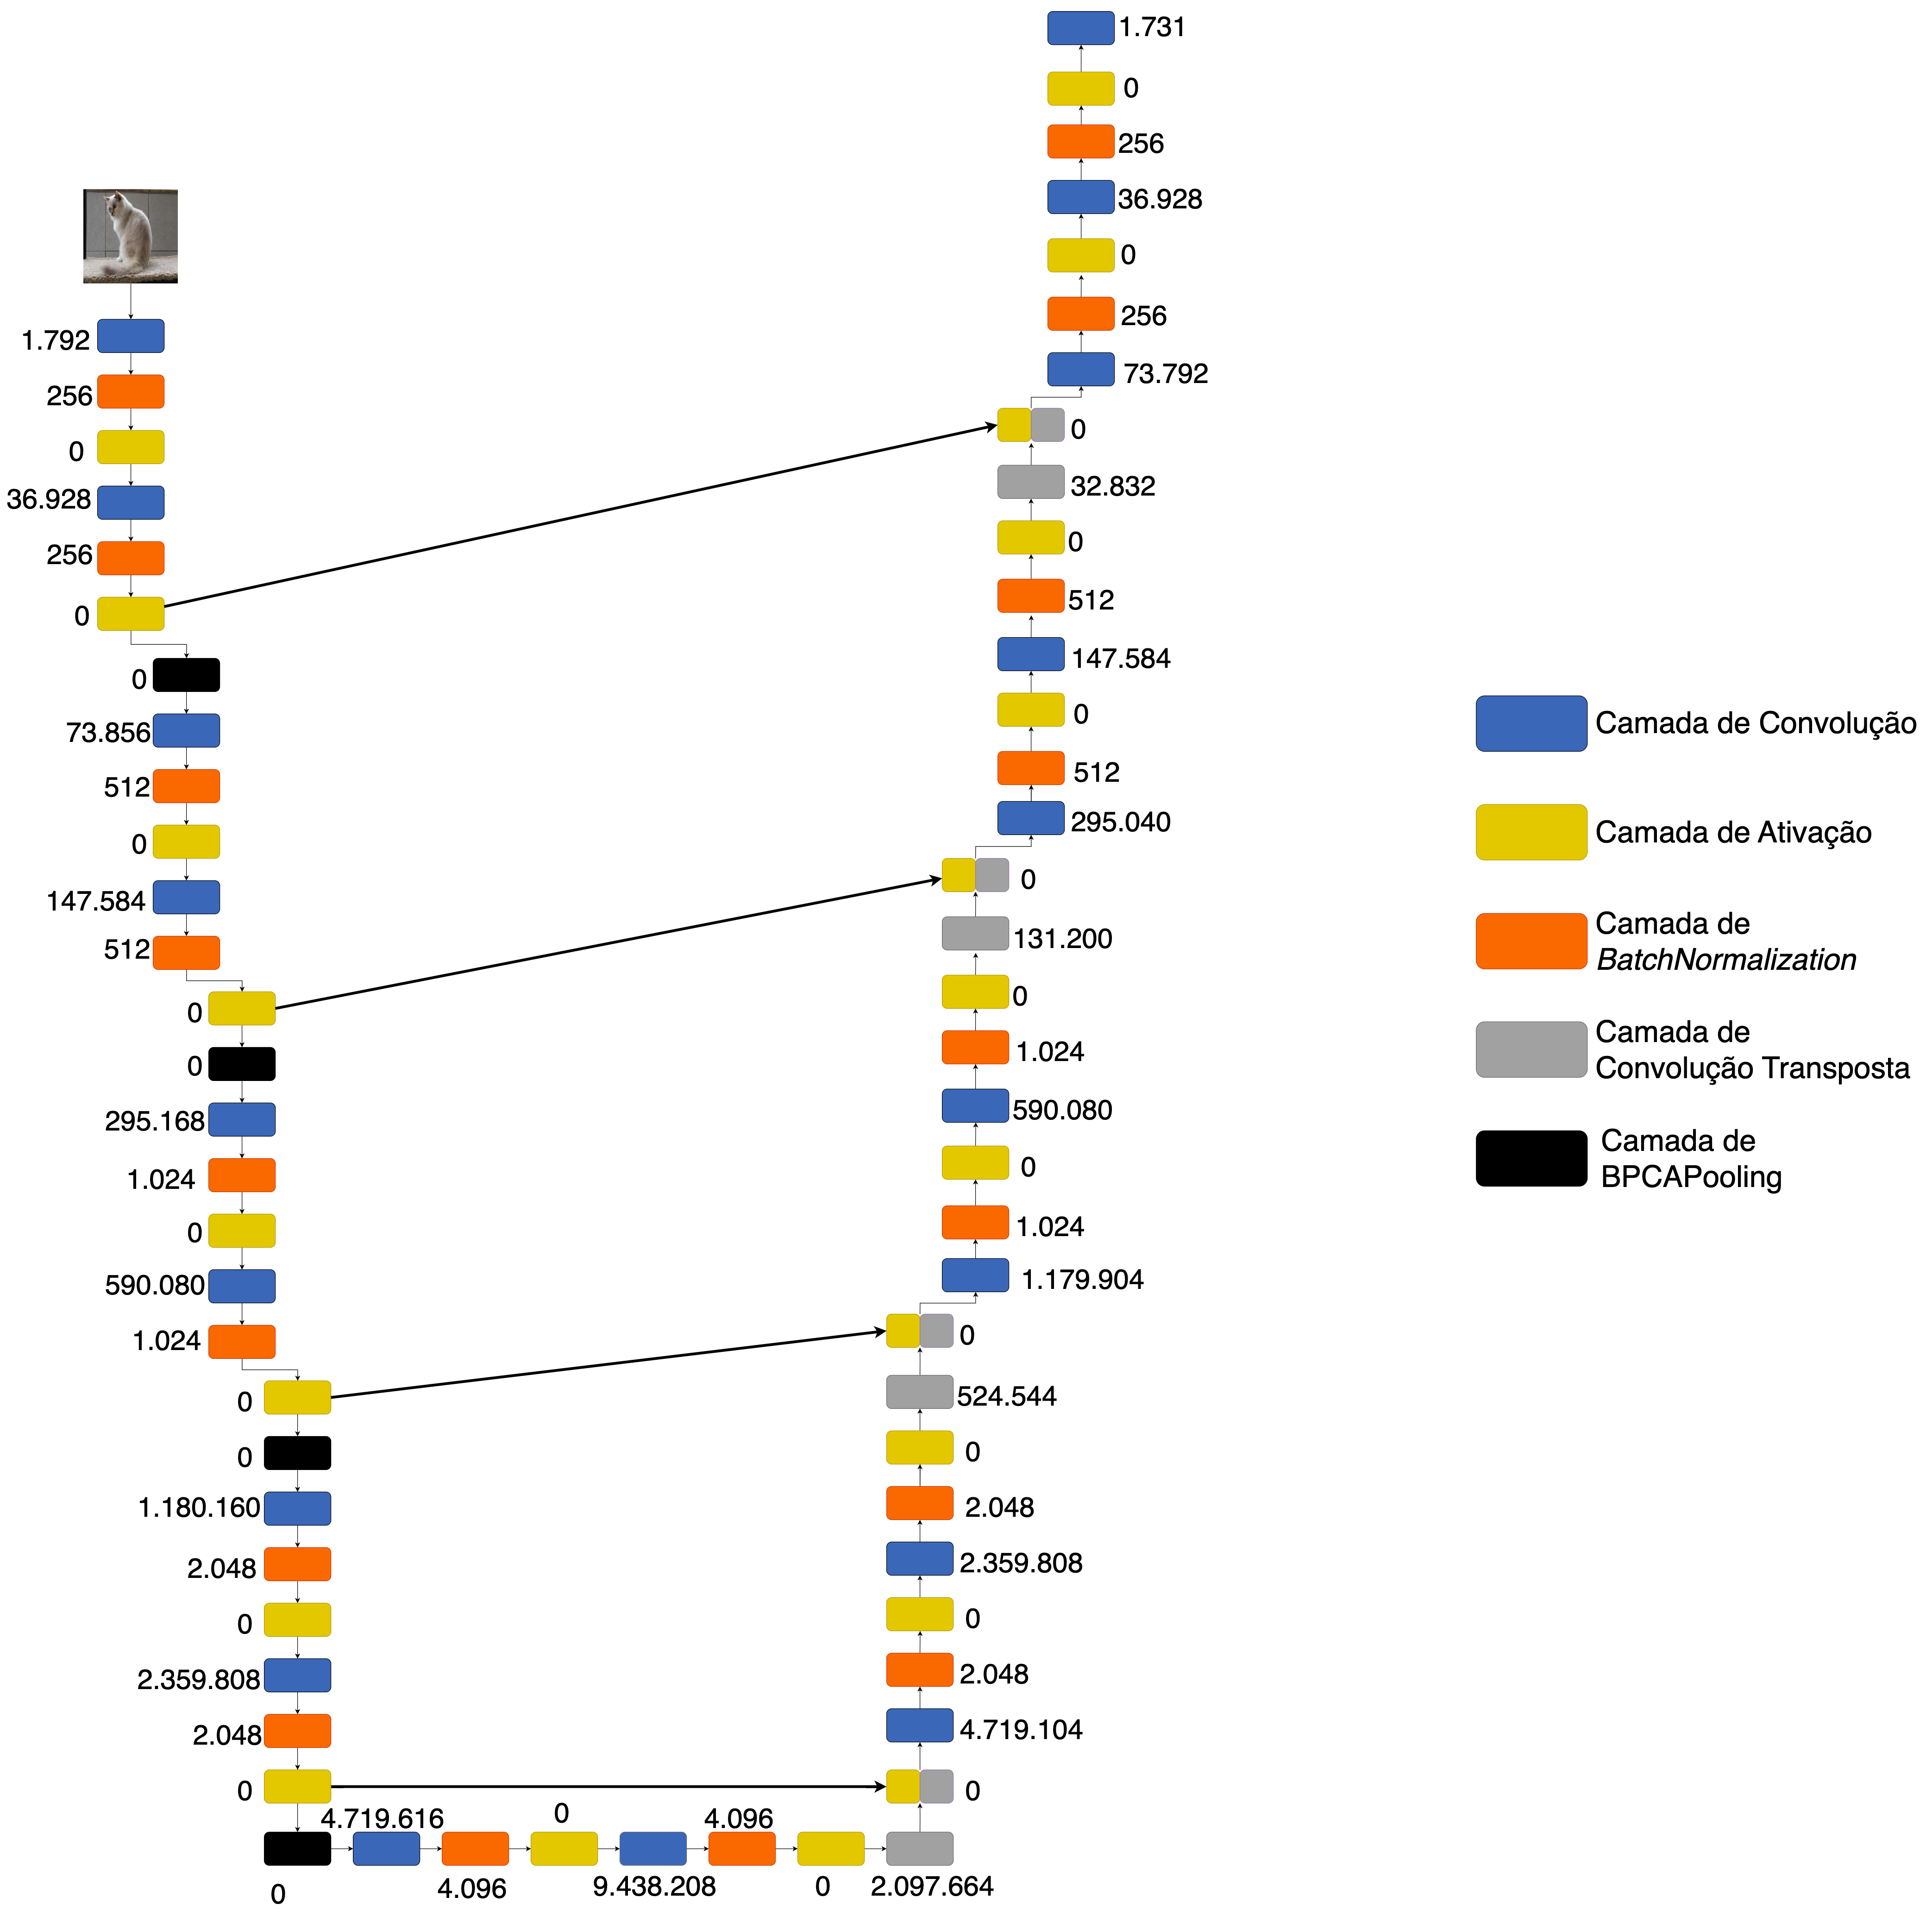
\includegraphics[width=1\textwidth]{recursos/imagens/project/unet-with-bpca.png}
    \label{project:fig:change_pooling:unet}

    Fonte: do próprio autor.
\end{figure}

A comparação entre as arquiteturas apresentadas nas Figuras \ref{project:fig:change_pooling:unet-like} e \ref{project:fig:change_pooling:unet} permite uma análise detalhada dos aspectos abordados na Seção \ref{semantic:arch}. A U-Net possui aproximadamente quinze vezes mais parâmetros do que a U-Net-\textit{Like}, totalizando $31.056.963$ parâmetros treináveis, enquanto a U-Net-\textit{Like} conta com $2.058.979$ parâmetros treináveis, considerando ambas as abordagens de \textit{pooling}. Notavelmente, os parâmetros do BPCAPooling permanecem zerados, seguindo o comportamento do \textit{Max Pooling}. Vale mencionar que a arquitetura U-Net-\textit{Like} inclui camadas de convolução separáveis e camadas de \textit{upsampling}. As camadas de \textit{upsampling} foram elucidadas na Seção \ref{semantic:unetlike}, enquanto as camadas convolucionais separáveis realizam convoluções espaciais profundas seguidas por uma convolução pontual, que mescla os canais de saída resultantes \citep{Zhao2018AutomaticFPGA}.


\subsection{Metodologia Experimental}
\label{project:exp_result}
Esta seção, busca elucidar as métricas de avaliação escolhidas para determinar o desempenho dos experimentos realizados neste estudo para atingir os objetivos mencionados na Seção \ref{intro:objectives}. Essas métricas são categorizadas em duas vertentes: classificação e segmentação semântica, que serão exploradas na Seção \ref{project:metrics}.

Com o intuito de promover a reproduzibilidade deste trabalho, oferece-se na Seção \ref{project:params} detalhes acerca dos parâmetros empregados no treinamento e testes conduzidos. Adicionalmente, na Seção \ref{project:explain}, será discorrido sobre as técnicas de explicabilidade de modelos de IA utilizadas neste estudo para melhor entender as classificações e segmentações à luz das percepções derivadas dos modelos.

\subsubsection{Escolha das Métricas}
\label{project:metrics}
Para a avaliação da VGG-16 nos processos de treinamento e teste nos conjuntos de dados CIFAR-100 e \textit{Food}-101, foram empregadas duas métricas: \textit{Sparse Categorical Crossentropy} para cálculo do erro e acurácia para avaliar o desempenho da rede. Essa métrica de erro é frequentemente utilizada em problemas de classificação multiclasse, como é o caso dos problemas nos conjuntos de dados mencionados, onde a saída é codificada de forma esparsa (categórica). Essa função de perda mede a diferença entre as previsões do modelo e os rótulos reais, penalizando as discrepâncias entre eles, conforme discutido na Seção \ref{deep:cust}. Essa função pode ser representada pela Equação \ref{project:eq:metrics1}:

\begin{equation}
    \label{project:eq:metrics1}
    J(\boldsymbol{w}) = - \sum_{i=1}^{N} y_i \cdot \text{log}(\hat{y}_i),
\end{equation}
em que $\boldsymbol{w}$ denota os parâmetros do modelo, $N$ é o número total de amostras, $y_i$ representa o rótulo real da amostra $i$, e $\hat{y}_i$ é a previsão do modelo para a amostra $i$.

Quanto à acurácia, discutida na Seção \ref{deep:metrics} e representada pela Equação \ref{deep:eq:13}, vale ressaltar que foi escolhida como métrica principal. Decisões durante o treinamento e teste, como o ponto de parada antecipado (Seção \ref{deep:optimization:early_stoping}), ajuste planejado da taxa de aprendizado (Seção \ref{deep:optimization:dynamic_lr}), seleção do melhor modelo, entre outros, foram baseadas no progresso dessa métrica.

Para avaliar as segmentações semânticas usando as arquiteturas U-Net-\textit{Like} e U-Net no conjunto de dados \textit{Oxford-IIIT Pets}, uma variedade de métricas foi empregada nos testes. Inicialmente, a métrica principal adotada foi a acurácia, conforme utilizado nos testes de classificação. Entretanto, o uso da métrica de acurácia é desencorajado para problemas de segmentação, já que muitos desses problemas podem enfrentar desequilíbrios entre as classes de interesse e o fundo \citep{Muller2022TowardsSegmentation}. Assim, a métrica principal adotada para os modelos de segmentação semântica passou a ser o \textit{Mean Intersection Over Union}, ou mIoU, detalhado na Seção \ref{semantic:miou}, representado pela Equação \ref{semantic:eq:miou}, superando as limitações da acurácia \citep{Muller2022TowardsSegmentation}.

Adicionalmente, com a adoção da métrica mIoU como métrica principal, incorporou-se o uso do \textit{Dice Similarity Coefficient} (DSC) mencionado na Seção \ref{semantic:f1}, para fornecer uma visão adicional sobre a performance dos modelos treinados. Quanto à métrica de função de custo empregada nos problemas de segmentação semântica, destaca-se que os desafios encontrados no conjunto de dados \textit{Oxford-IIIT Pets} são semelhantes aos encontrados nos \textit{datasets} de classificação mencionados anteriormente nesta seção. Portanto, a métrica \textit{Sparse Categorical Crossentropy} continuou a ser utilizada.

Em suma, a seleção apropriada de métricas para avaliar o desempenho dos modelos de aprendizagem profunda é crítica para fornecer uma demonstração adequada de seu desempenho e adaptabilidade a diferentes tarefas. Nos experimentos realizados neste estudo, optou-se por uma combinação de métricas apropriadas para tarefas de classificação e segmentação semântica com base nas especificações únicas atribuídas a cada tarefa. O uso rigoroso e bem planejado dessas métricas por meio da hipótese orientada aumentou a robustez e a credibilidade dos resultados obtidos. A lista completa de métricas utilizadas, assim como suas aplicações, é chave para observar uma ótima otimização dos parâmetros do modelo de aprendizagem e, assim, atingir uma interpretação ideal da tarefa variada que o modelo é treinado para resolver.


\subsubsection{Parâmetros de Treinamento e Teste}
\label{project:params}
Nessa Seção serão esmiuçados os detalhes dos parâmetros utilizados para o treinamento e teste das redes neurais. Esta investigação contemplará tanto os experimentos voltados à classificação, que empregaram a arquitetura da VGG-16 nos conjuntos de dados \textit{Food}-101 e CIFAR 100, quanto aqueles destinados à segmentação semântica. No caso da segmentação, exploramos as arquiteturas U-Net-\textit{Like} e U-Net aplicadas no conjunto de dados \textit{Oxford-IIIT Pets}.

Os parâmetros de treinamento e teste são de extrema importância no desenvolvimento de um modelo, uma vez que eles determinam o comportamento do aprendizado da rede. Aqui, buscaremos elucidar como a seleção destes parâmetros foi realizada para os diferentes cenários de nossa pesquisa. Deste modo, permitiremos que futuras pesquisas na área possam ser facilmente replicáveis ou até mesmo aprimoradas, através do ajuste destes parâmetros.

\paragraph{VGG-16 + \textit{Food}-101}
\label{params:vggfood}
Na configuração da VGG-16 para o conjunto de dados \textit{Food}-101, é relevante destacar a definição inicial das sementes (\textit{seeds}) foram iguais à $77$ para as bibliotecas TensorFlow e NumPy, valor o qual foi escolhido empiricamente. Essas sementes foram estabelecidas visando a reprodução consistente dos resultados nos testes, reduzindo variações indesejadas \citep{Alahmari2020ChallengesModels}. Além disso, durante a fase de preparação dos dados, um parâmetro crucial foi o tamanho do lote (\textit{batch size}), estabelecido em $64$. Este parâmetro determina a quantidade de imagens usadas no treinamento durante uma única época \citep{Kandel2020TheDataset}. Por fim, entre as variáveis mantidas constantes em todos os procedimentos, destaca-se a taxa de aprendizado definida como $1e^{-5}$, considerada uma taxa mais conservadora, cuja importância é discutida na Seção \ref{deep:optimization:dynamic_lr}.

Outros parâmetros relevantes incluem o número de épocas usadas para treinamento e teste do modelo, bem como as funções de otimização empregadas nesses processos. Adicionalmente, a estratégia de atualização dinâmica da taxa de aprendizado com CLR \citep{Smith2017CyclicalNetworks} é digna de menção. No entanto, devido à realização de um processo de ajuste fino (\textit{fine-tuning}) nas arquiteturas da VGG-16, é importante ressaltar que esses parâmetros variavam de acordo com a fase da execução. Cada modelo foi treinado quatro vezes, como ilustrado na Figura \ref{project:fig:transf1} e mencionado na Seção \ref{project:transf}. Portanto, as Tabelas \ref{project:tab:params:vggfoodbpca}, \ref{project:tab:params:vggfoodmax} e \ref{project:tab:params:vggfoodavg} apresentam os parâmetros utilizados em cada fase do processo de \textit{fine-tuning} com o uso de BPCAPooling, \textit{Max Pooling} e \textit{Avg Pooling}, respectivamente.

\begin{table}[H]
    \centering
    \caption{Parâmetros de treinamento e teste com VGG-16 e BPCAPooling no conjunto \textit{Food}-101.}
    \label{project:tab:params:vggfoodbpca}
    \resizebox{1\textwidth}{!}{
        \begin{tabular}{l|l|l|l|l|l|l|l|l}
            % \firsthline
            \multicolumn{1}{c|}{\textbf{Parâmetros}}      & \multicolumn{2}{c|}{\textbf{\textit{Warm-up}}}                                          & \multicolumn{2}{c|}{\textbf{Bloco 5}}                                          & \multicolumn{2}{c|}{\textbf{Bloco 4}}                                          & \multicolumn{2}{c}{\textbf{Bloco 3}}     \\
            \cline{2-9}
            \multicolumn{1}{c|}{\textbf{}}                & \multicolumn{1}{c|}{\textbf{Valor}} & \multicolumn{1}{c|}{\textbf{Uso}} & \multicolumn{1}{c|}{\textbf{Valor}} & \multicolumn{1}{c|}{\textbf{Uso}} & \multicolumn{1}{c|}{\textbf{Valor}} & \multicolumn{1}{c|}{\textbf{Uso}} & \multicolumn{1}{c|}{\textbf{Valor}} & \multicolumn{1}{c}{\textbf{Uso}} \\
            \hline
            Épocas                                       & 700                                & -                       & 700                                & -                       & 700                                & -                       & 700                                & -                                                                  \\
            Época de Parada                              & 188                                & -                       & 167                                & -                       & 700                                & -                       & 219                                & -                                                                  \\
            Parada Antecipada                            & -                                  & Verdadeiro              & -                                  & Verdadeiro              & -                                  & Verdadeiro              & -                                  & Verdadeiro                                                         \\
            CLR                                          & -                                  & Falso                   & -                                  & Verdadeiro              & -                                  & Verdadeiro              & -                                  & Verdadeiro                                                         \\
            Taxa de Aprendizado Mínima                   & 0,0001                             & -                       & 0,00001                            & -                       & 0,00001                            & -                       & 0,00001                            & -                                                                  \\
            Taxa de Aprendizado Máxima                   & 0,0001                             & -                       & 0,0001                             & -                       & 0,0001                             & -                       & 0,0001                             & -                                                                  \\
            Função de Otimização                         & Adam                               & -                       & SGD                                & -                       & SGD                                & -                       & SGD                                & -                       
        \end{tabular}
        }

    \vspace*{1 cm}
    Fonte: do próprio autor.
\end{table}


\begin{table}[H]
    \centering
    \caption{Parâmetros de treinamento e teste com VGG-16 e \textit{Max Pooling} no conjunto \textit{Food}-101.}
    \label{project:tab:params:vggfoodmax}
    \resizebox{1\textwidth}{!}{
        \begin{tabular}{l|l|l|l|l|l|l|l|l}
            % \firsthline
            \multicolumn{1}{c|}{\textbf{Parâmetros}}      & \multicolumn{2}{c|}{\textbf{\textit{Warm-up}}}                                          & \multicolumn{2}{c|}{\textbf{Bloco 5}}                                          & \multicolumn{2}{c|}{\textbf{Bloco 4}}                                          & \multicolumn{2}{c}{\textbf{Bloco 3}}     \\
            \cline{2-9}
            \multicolumn{1}{c|}{\textbf{}}                & \multicolumn{1}{c|}{\textbf{Valor}} & \multicolumn{1}{c|}{\textbf{Uso}} & \multicolumn{1}{c|}{\textbf{Valor}} & \multicolumn{1}{c|}{\textbf{Uso}} & \multicolumn{1}{c|}{\textbf{Valor}} & \multicolumn{1}{c|}{\textbf{Uso}} & \multicolumn{1}{c|}{\textbf{Valor}} & \multicolumn{1}{c}{\textbf{Uso}} \\
            \hline
            Épocas                                       & 700                                & -                       & 700                                & -                       & 700                                & -                       & 700                                & -                                                                  \\
            Época de Parada                              & 700                                & -                       & 700                                & -                       & 514                                & -                       & 105                                & -                                                                  \\
            Parada Antecipada                            & -                                  & Falso                   & -                                  & Falso                   & -                                  & Verdadeiro              & -                                  & Verdadeiro                                                         \\
            CLR                                          & -                                  & Falso                   & -                                  & Verdadeiro              & -                                  & Verdadeiro              & -                                  & Verdadeiro                                                         \\
            Taxa de Aprendizado Mínima                   & 0.0001                             & -                       & 0.00001                            & -                       & 0.00001                            & -                       & 0.00001                            & -                                                                  \\
            Taxa de Aprendizado Máxima                   & 0.0001                             & -                       & 0.0001                             & -                       & 0.0001                             & -                       & 0.0001                             & -                                                                  \\
            Função de Otimização                         & Adam                               & -                       & SGD                                & -                       & SGD                                & -                       & SGD                                & -                       
        \end{tabular}
        }

    \vspace*{1 cm}
    Fonte: do próprio autor.
\end{table}


\begin{table}[H]
    \centering
    \caption{Parâmetros de treinamento e teste com VGG-16 e \textit{Avg Pooling} no conjunto \textit{Food}-101.}
\label{project:tab:params:vggfoodavg}
\resizebox{1\textwidth}{!}{
    \begin{tabular}{l|l|l|l|l|l|l|l|l}
        % \firsthline
        \multicolumn{1}{c|}{\textbf{Parâmetros}}      & \multicolumn{2}{c|}{\textbf{\textit{Warm-up}}}                                          & \multicolumn{2}{c|}{\textbf{Bloco 5}}                                          & \multicolumn{2}{c|}{\textbf{Bloco 4}}                                          & \multicolumn{2}{c}{\textbf{Bloco 3}}     \\
        \cline{2-9}
        \multicolumn{1}{c|}{\textbf{}}                & \multicolumn{1}{c|}{\textbf{Valor}} & \multicolumn{1}{c|}{\textbf{Uso}} & \multicolumn{1}{c|}{\textbf{Valor}} & \multicolumn{1}{c|}{\textbf{Uso}} & \multicolumn{1}{c|}{\textbf{Valor}} & \multicolumn{1}{c|}{\textbf{Uso}} & \multicolumn{1}{c|}{\textbf{Valor}} & \multicolumn{1}{c}{\textbf{Uso}} \\
        \hline
        Épocas                                       & 700                                & -                       & 700                                & -                       & 700                                & -                       & 700                                & -                                                                  \\
        Época de Parada                              & 700                                & -                       & 700                                & -                       & 700                                & -                       & 249                                & -                                                                  \\
        Parada Antecipada                            & -                                  & Falso                   & -                                  & Falso                   & -                                  & Verdadeiro              & -                                  & Verdadeiro                                                         \\
        CLR                                          & -                                  & Falso                   & -                                  & Verdadeiro              & -                                  & Verdadeiro              & -                                  & Verdadeiro                                                         \\
        Taxa de Aprendizado Mínima                   & 0,0001                             & -                       & 0,00001                            & -                       & 0,00001                            & -                       & 0,00001                            & -                                                                  \\
        Taxa de Aprendizado Máxima                   & 0,0001                             & -                       & 0,0001                             & -                       & 0,0001                             & -                       & 0,0001                             & -                                                                  \\
        Função de Otimização                         & Adam                               & -                       & SGD                                & -                       & SGD                                & -                       & SGD                                & -                       
    \end{tabular}
    }

\vspace*{1 cm}
Fonte: do próprio autor.
\end{table}

Analisando as Tabelas \ref{project:tab:params:vggfoodbpca}, \ref{project:tab:params:vggfoodmax} e \ref{project:tab:params:vggfoodavg}, observa-se que o parâmetro que mais se destaca é a Época de Parada, o qual é influenciado pela técnica de Parada Antecipada (\textit{Early Stopping}). Ademais, as variações entre as configurações se dão pelo emprego ou não da taxa de aprendizado dinâmica utilizando o método CLR (\textit{Cyclical Learning Rate}). Essas discrepâncias refletem diferentes estratégias adotadas no treinamento dos modelos.

\paragraph{VGG-16 + CIFAR 100}
\label{params:vggcifar}
A abordagem aplicada na combinação da VGG-16 com o conjunto de dados CIFAR-100 segue um padrão semelhante à utilizada na combinação da VGG-16 com o conjunto de dados \textit{Food}-101, com relação ao uso das técnicas. Dentre os parâmetros mantidos constantes durante o processo, destaca-se a taxa de aprendizado máxima, o tamanho do lote (\textit{batch size}) e o número de épocas, estabelecidos em $1e^{-5}$, $64$, e $700$, respectivamente. Quanto às outras variáveis, os valores específicos podem ser visualizados detalhadamente nas Tabelas \ref{project:tab:params:vggcifarbpca}, \ref{project:tab:params:vggcifarmax} e \ref{project:tab:params:vggcifaravg}, para as configurações de BPCAPooling, \textit{Max Pooling} e \textit{Avg Pooling}, respectivamente.


\begin{table}[H]
    \centering
    \caption{Parâmetros de treinamento e teste com VGG-16 e BPCAPooling no conjunto CIFAR 100.}
\label{project:tab:params:vggcifarbpca}
\resizebox{1\textwidth}{!}{
    \begin{tabular}{l|l|l|l|l|l|l|l|l}
        % \firsthline
        \multicolumn{1}{c|}{\textbf{Parâmetros}}      & \multicolumn{2}{c|}{\textbf{\textit{Warm-up}}}                                          & \multicolumn{2}{c|}{\textbf{Bloco 5}}                                          & \multicolumn{2}{c|}{\textbf{Bloco 4}}                                          & \multicolumn{2}{c}{\textbf{Bloco 3}}     \\
        \cline{2-9}
        \multicolumn{1}{c|}{\textbf{}}                & \multicolumn{1}{c|}{\textbf{Valor}} & \multicolumn{1}{c|}{\textbf{Uso}} & \multicolumn{1}{c|}{\textbf{Valor}} & \multicolumn{1}{c|}{\textbf{Uso}} & \multicolumn{1}{c|}{\textbf{Valor}} & \multicolumn{1}{c|}{\textbf{Uso}} & \multicolumn{1}{c|}{\textbf{Valor}} & \multicolumn{1}{c}{\textbf{Uso}} \\
        \hline
        Épocas                                       & 700                                & -                       & 700                                & -                       & 700                                & -                       & 700                                & -                                                                  \\
        Época de Parada                              & 700                                & -                       & 700                                & -                       & 473                                & -                       & 700                                & -                                                                  \\
        Parada Antecipada                            & -                                  & Falso                   & -                                  & Falso                   & -                                  & Verdadeiro              & -                                  & Verdadeiro                                                         \\
        CLR                                          & -                                  & Falso                   & -                                  & Verdadeiro              & -                                  & Verdadeiro              & -                                  & Verdadeiro                                                         \\
        Taxa de Aprendizado Mínima                   & 0,0001                             & -                       & 0,00001                            & -                       & 0,00001                            & -                       & 0,00001                            & -                                                                  \\
        Taxa de Aprendizado Máxima                   & 0,0001                             & -                       & 0,0001                             & -                       & 0,0001                             & -                       & 0,0001                             & -                                                                  \\
        Função de Otimização                         & Adam                               & -                       & SGD                                & -                       & SGD                                & -                       & SGD                                & -                       
    \end{tabular}
    }

\vspace*{1 cm}
Fonte: do próprio autor.
\end{table}


\begin{table}[H]
    \centering
    \caption{Parâmetros de treinamento e teste com VGG-16 e \textit{Max Pooling} no conjunto CIFAR 100.}
\label{project:tab:params:vggcifarmax}
\resizebox{1\textwidth}{!}{
    \begin{tabular}{l|l|l|l|l|l|l|l|l}
        % \firsthline
        \multicolumn{1}{c|}{\textbf{Parâmetros}}      & \multicolumn{2}{c|}{\textbf{\textit{Warm-up}}}                                          & \multicolumn{2}{c|}{\textbf{Bloco 5}}                                          & \multicolumn{2}{c|}{\textbf{Bloco 4}}                                          & \multicolumn{2}{c}{\textbf{Bloco 3}}     \\
        \cline{2-9}
        \multicolumn{1}{c|}{\textbf{}}                & \multicolumn{1}{c|}{\textbf{Valor}} & \multicolumn{1}{c|}{\textbf{Uso}} & \multicolumn{1}{c|}{\textbf{Valor}} & \multicolumn{1}{c|}{\textbf{Uso}} & \multicolumn{1}{c|}{\textbf{Valor}} & \multicolumn{1}{c|}{\textbf{Uso}} & \multicolumn{1}{c|}{\textbf{Valor}} & \multicolumn{1}{c}{\textbf{Uso}} \\
        \hline
        Épocas                                       & 700                                & -                       & 700                                & -                       & 700                                & -                       & 700                                & -                                                                  \\
        Época de Parada                              & 700                                & -                       & 700                                & -                       & 700                                & -                       & 550                                & -                                                                  \\
        Parada Antecipada                            & -                                  & Falso                   & -                                  & Falso                   & -                                  & Verdadeiro              & -                                  & Verdadeiro                                                         \\
        CLR                                          & -                                  & Falso                   & -                                  & Verdadeiro              & -                                  & Verdadeiro              & -                                  & Verdadeiro                                                         \\
        Taxa de Aprendizado Mínima                   & 0,0001                             & -                       & 0,00001                            & -                       & 0,00001                            & -                       & 0,00001                            & -                                                                  \\
        Taxa de Aprendizado Máxima                   & 0,0001                             & -                       & 0,0001                             & -                       & 0,0001                             & -                       & 0,0001                             & -                                                                  \\
        Função de Otimização                         & Adam                               & -                       & SGD                                & -                       & SGD                                & -                       & SGD                                & -                       
    \end{tabular}
    }

\vspace*{1 cm}
Fonte: do próprio autor.
\end{table}


\begin{table}[H]
    \centering
    \caption{Parâmetros de treinamento e teste com VGG-16 e \textit{Avg Pooling} no conjunto CIFAR 100.}
\label{project:tab:params:vggcifaravg}
\resizebox{1\textwidth}{!}{
    \begin{tabular}{l|l|l|l|l|l|l|l|l}
        % \firsthline
        \multicolumn{1}{c|}{\textbf{Parâmetros}}      & \multicolumn{2}{c|}{\textbf{\textit{Warm-up}}}                                          & \multicolumn{2}{c|}{\textbf{Bloco 5}}                                          & \multicolumn{2}{c|}{\textbf{Bloco 4}}                                          & \multicolumn{2}{c}{\textbf{Bloco 3}}     \\
        \cline{2-9}
        \multicolumn{1}{c|}{\textbf{}}                & \multicolumn{1}{c|}{\textbf{Valor}} & \multicolumn{1}{c|}{\textbf{Uso}} & \multicolumn{1}{c|}{\textbf{Valor}} & \multicolumn{1}{c|}{\textbf{Uso}} & \multicolumn{1}{c|}{\textbf{Valor}} & \multicolumn{1}{c|}{\textbf{Uso}} & \multicolumn{1}{c|}{\textbf{Valor}} & \multicolumn{1}{c}{\textbf{Uso}} \\
        \hline
        Épocas                                       & 700                                & -                       & 700                                & -                       & 700                                & -                       & 700                                & -                                                                  \\
        Época de Parada                              & 700                                & -                       & 700                                & -                       & 700                                & -                       & 350                                & -                                                                  \\
        Parada Antecipada                            & -                                  & Falso                   & -                                  & Falso                   & -                                  & Falso                   & -                                  & Verdadeiro                                                         \\
        CLR                                          & -                                  & Falso                   & -                                  & Verdadeiro              & -                                  & Verdadeiro              & -                                  & Verdadeiro                                                         \\
        Taxa de Aprendizado Mínima                   & 0,0001                             & -                       & 0,00001                            & -                       & 0,00001                            & -                       & 0,00001                            & -                                                                  \\
        Taxa de Aprendizado Máxima                   & 0,0001                             & -                       & 0,0001                             & -                       & 0,0001                             & -                       & 0,0001                             & -                                                                  \\
        Função de Otimização                         & Adam                               & -                       & SGD                                & -                       & SGD                                & -                       & SGD                                & -                       
    \end{tabular}
    }

\vspace*{1 cm}
Fonte: do próprio autor.
\end{table}


\paragraph{U-Net-\textit{Like} + \textit{Oxford-IIIT Pets}}
\label{params:unetlikepets}
Na configuração dos parâmetros para a arquitetura U-Net-\textit{Like} aplicada ao conjunto de dados \textit{Oxford-IIIT Pets}, é importante observar que não foi realizado um processo de \textit{fine-tuning}, diferentemente das arquiteturas utilizadas para classificação que foram mencionadas anteriormente. No entanto, muitos dos parâmetros se mantiveram consistentes. Neste contexto, foram adotadas sementes para as bibliotecas TensorFlow e Numpy, com um valor empírico de $77$, garantindo a reprodutibilidade dos testes.

Para a U-Net-\textit{Like}, foram realizados treinamentos e testes ao longo de $20$ e $500$ épocas, respectivamente, antecedendo os experimentos relacionados à arquitetura U-Net, a qual será discutida na Seção \ref{params:unetpets}. Em relação à taxa de aprendizado máxima, vale ressaltar que seu valor foi mantido constante em $1 \times 10^{-4}$ para todos os experimentos realizados. Apesar de parecer uma taxa mais elevada em comparação com as anteriores, está dentro do limite recomendado quando comparado com outras pesquisas \citep{Fajar2023CyclicalSegmentation}. Além disso, a taxa de aprendizado mínima foi definida como $1 \times 10^{-5}$, sendo reduzida quando o modelo não apresentou evolução na métrica de avaliação principal após $25$ épocas para os testes com $500$ épocas, pois para os de $20$ épocas a redução não foi utilizada. Em relação ao valor do \textit{batch size}, esse se manteve constante em $64$, seguindo o padrão dos experimentos anteriores com a rede VGG-16.

Em contraste com os experimentos anteriores, foram utilizadas fórmulas para calcular a quantidade de iterações por época, conforme representado pela Equação \ref{params:eq1:unetlikepets}, e para calcular a quantidade das iterações de validação, representadas pela Equação \ref{params:eq2:unetlikepets}, descritas respectivamente por:

\begin{equation}
    \label{params:eq1:unetlikepets}
    \text{Passos por Época} = \frac{\text{tamanho do conjunto de treino}}{\text{tamanho do lote}}
\end{equation}

e

\begin{equation}
    \label{params:eq2:unetlikepets}
    \text{Passos de Validação} = \frac{\text{tamanho do conjunto de teste}}{\text{tamanho do lote}} \cdot \frac{1}{\text{divisões de validação}},
\end{equation}
onde que as divisões de validação foram definidas manualmente, sendo que essas divisões de validação foram definidas manualmente com o valor de $5$, representando a quantidade de partes em que o conjunto de validação foi dividido para avaliações separadas durante o treinamento. Esse método permite uma validação cruzada interna durante o processo de treinamento, o que contribui para uma avaliação mais robusta do modelo ao longo das épocas. Essa abordagem de validação cruzada ajuda a monitorar a performance e o ajuste do modelo, oferecendo\textit{ insights }valiosos sobre o seu desempenho geral. Os valores obtidos foram de $57$ passos por época e $9$ passos de validação.

Por fim, é importante ressaltar que o otimizador Adam foi utilizado de forma unânime em todos os testes realizados. Essa escolha se justifica pelo fato de que, sem a aplicação do processo de \textit{fine-tuning}, a variação da função de otimização não é habitualmente realizada. Dessa maneira, optou-se por manter o otimizador Adam constante em todos os experimentos, visando uma maior consistência nos resultados obtidos.


\paragraph{U-Net + \textit{Oxford-IIIT Pets}}
\label{params:unetpets}
No último experimento realizado, a arquitetura da U-Net foi combinada com os métodos de \textit{pooling} BPCAPooling e \textit{Max Pooling} em um treinamento de $500$ épocas. É importante mencionar que a U-Net é considerada uma rede mais robusta, possuindo um número significativo de parâmetros (vide Seção \ref{project:change_pooling}), o que impacta diretamente no tempo e nos recursos computacionais necessários para o treinamento e teste.

Assim como nos experimentos anteriores com a arquitetura U-Net-\textit{Like}, o otimizador Adam foi utilizado de forma constante. A taxa de aprendizado mínima foi mantida em $1 \times 10^{-5}$, enquanto a taxa de aprendizado máxima foi definida como $1 \times 10^{-4}$. A estratégia de redução da taxa de aprendizado foi aplicada após $25$ épocas sem melhora na métrica principal.

O critério de parada antecipada foi mantido constante em todos os experimentos realizados. A utilização das Equações \ref{params:eq1:unetlikepets} e \ref{params:eq2:unetlikepets} também foi aplicada nos experimentos da U-Net, resultando em $18$ passos de validação e $115$ passos por época, visto que as divisões de validação mantiveram-se no valor de $5$.

Por fim, é relevante destacar que o valor da semente permaneceu empiricamente em $77$ para garantir a reprodutibilidade dos resultados. No entanto, o tamanho do lote teve que ser reduzido para $32$, uma vez que o \textit{hardware}, apesar de possuir $24.564$ MiB, não suportava o uso do parâmetro igual a $64$, como feito nos demais testes.


\subsubsection{Explicabilidade de Modelos}
\label{project:explain}
No contexto da explicação de modelos, abordaremos o uso de ferramentas pertencentes à área de Inteligência Artificial Explicável, também conhecida como \textit{Explainable Artificial Intelligence} (XAI) \citep{Gunning2019XAIExplainableIntelligence}. Essa área visa mitigar as limitações dos modelos de \quotes{caixa-preta}, tornando-os mais compreensíveis para os humanos, elucidando seu funcionamento de maneira mais transparente e interpretável \citep{Angelov2021ExplainableReview}.

No decorrer dos experimentos com os modelos de classificação, aplicou-se o LIME, acrônimo para \textit{Local Interpretable Model-Agnostic Explanations}, uma técnica desenvolvida por \cite{Ribeiro2016WhyClassifier}. O LIME oportuniza entender as previsões de classificadores de uma maneira intuitiva, ao identificar as regiões críticas de uma imagem que mais contribuem para a decisão do modelo.

O mecanismo do LIME baseia-se em aproximar o modelo original, em um determinado ponto de interesse, com um modelo linear interpretável localmente. Este processo é conduzido por meio da geração de novas amostras com perturbações ao redor do ponto de interesse, classificando-as com o uso do modelo original, e então ajustando um modelo linear com base na saída \citep{Ribeiro2016WhyClassifier}. As características mais relevantes, aquelas que contribuem mais para a tomada de decisão, são destacadas na imagem, proporcionando um entendimento de qual influência cada parte da imagem tem na decisão final do modelo.

Ao se empregar essa perspectiva oferecida pelo LIME, observam-se as áreas de maior influência na classificação ressaltadas na imagem, tornando possível averiguar se a decisão do modelo é impactada pelo contexto da imagem, como o fundo, ou por elementos não pertinentes à classificação correta. Um exemplo ilustrativo dessa situação é demonstrado na Figura \ref{project:fig:explain:lime1}. Neste caso, o modelo confundiu um cachorro Husky com um lobo, dado que o fundo nevado no contexto da imagem é um ambiente comumente associado a fotos de lobos. Esta análise, viabilizada pela interpretabilidade proporcionada pelo LIME, auxilia em evidenciar e entender as falhas do modelo.

\begin{figure}[H]
    \centering
    \caption{Exemplo de saída gerado pelo LIME em situação de erro.}
    \label{project:fig:explain:lime1}
    \begin{subfigure}[t]{0.45\textwidth}
        \centering
        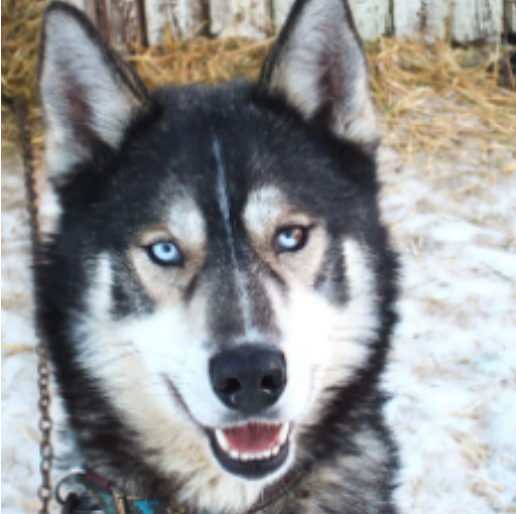
\includegraphics[width=1\linewidth]{recursos/imagens/project/husky.png}
        \caption{Cachorro Husky identificado erroneamente como Lobo.}
        \label{project:fig:explain:lime1.1}
    \end{subfigure}%
    ~
    \begin{subfigure}[t]{0.45\textwidth}
        \centering
        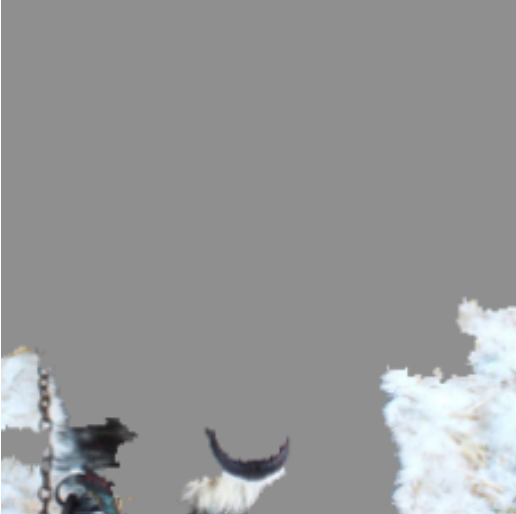
\includegraphics[width=1\linewidth]{recursos/imagens/project/fundo_husky.png}
        \caption{Destaque na explicação da predição.}
        \label{project:fig:explain:lime1.2}
    \end{subfigure}%

    Fonte: retirado e adaptado de \cite{Ribeiro2016WhyClassifier}.
\end{figure}

Idealmente, o LIME destaca partes da imagem diretamente associadas às regiões do objeto que influenciam a inferência do modelo, oferecendo informações cruciais sobre o processo de tomada de decisão do modelo, conforme ilustrado na Figura \ref{project:fig:explain:lime2}.

\begin{figure}[H]
    \centering
    \caption{Exemplo de saída gerado pelo LIME em situação correta.}
    \label{project:fig:explain:lime2}
    \begin{subfigure}[t]{0.45\textwidth}
        \centering
        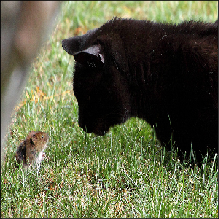
\includegraphics[width=1\linewidth]{recursos/imagens/project/gato.png}
        \caption{Classificação correta do \quotes{Gato} como \quotes{gato}.}
        \label{project:fig:explain:lime2.1}
    \end{subfigure}%
    ~
    \begin{subfigure}[t]{0.45\textwidth}
        \centering
        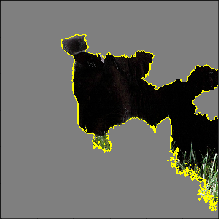
\includegraphics[width=1\linewidth]{recursos/imagens/project/mascara_gato.png}
        \caption{Destaque na explicação da predição.}
        \label{project:fig:explain:lime2.2}
    \end{subfigure}%

    Fonte: retirado e adaptado de \cite{Ribeiro2016WhyClassifier}.
\end{figure}

Contudo, ao tentar aplicar os conceitos de \textit{Explainable AI} (XAI) com o uso do LIME em problemas de segmentação semântica, não se obteve sucesso, uma vez que todos os pixels nessas segmentações representam áreas de interesse. Diante dessa limitação, recorreu-se ao \textit{framework} Xplique \citep{Fel2022}, que, dentre suas funcionalidades, utiliza da aplicação de métodos de atribuição destinados a produzir mapas de calor (\textit{heatmaps}) com o intuito de explicar as áreas de foco dos modelos em relação às instâncias segmentadas \citep{Fel2022}. Essa abordagem assemelha-se ao propósito do LIME e a aplicação dos métodos de atribuição evidenciando áreas de maior influencia mapeadas pelo modelo, por meio de mapas de calor, podem ser visualizados na Figura \ref{project:fig:explain:xplique}.

\begin{figure}[H]
    \centering
    \caption{Exemplo de aplicação de métodos de atribuição da ferramenta Xplique.}
    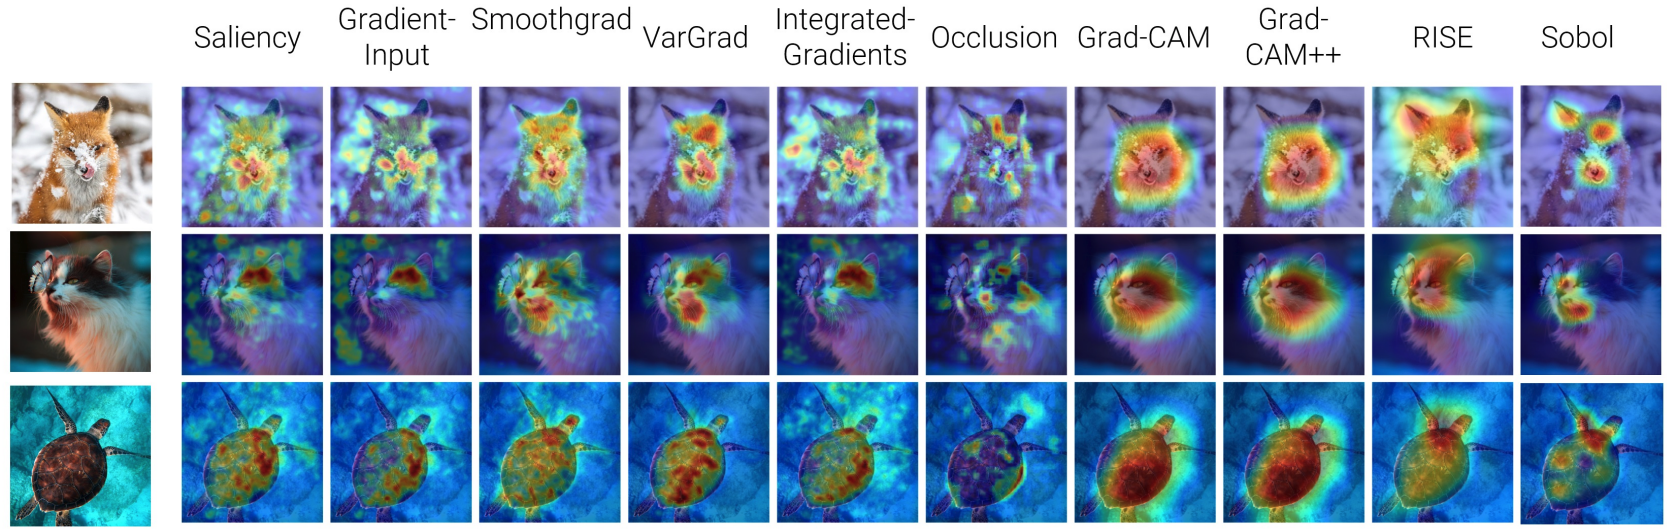
\includegraphics[width=1\textwidth]{recursos/imagens/project/xplique.png}
    \label{project:fig:explain:xplique}

    Fonte: retirado e adaptado de \cite{Fel2022}.
\end{figure}

Por fim, é evidente que a incorporação de ferramentas de Inteligência Artificial Explicável (XAI) proporciona \textit{insights} cruciais sobre a dinâmica interna dos modelos de aprendizagem profunda. A capacidade de revelar as regiões da imagem de entrada que mais influenciam as predições do modelo, viabilizada pelo uso do LIME e do Xplique, oferece uma visão mais detalhada do processo interpretativo dos modelos. Assim, a adoção dessas abordagens explanatórias não apenas promove a confiança nos modelos de Aprendizado Profundo, mas também aprimora sua compreensibilidade, aspectos essenciais tanto em aplicações do mundo real quanto em propostas de pesquisas futuras.

As descobertas e desafios enfrentados durante a utilização dessas técnicas serão minuciosamente explorados no Capítulo \ref{results}, o qual se dedica a apresentar os resultados dos experimentos em profundidade.

% \subsection{Revisão de Literatura}
% \label{project:revision}
% A revisão sistemática é uma metodologia robusta amplamente aplicada em diferentes campos científicos, particularmente em pesquisa clínica e médica. Com suas características de redução de viés e fornecimento de uma crítica abrangente da literatura existente, ela oferece um grau elevado de confiabilidade \citep{barbosa2019}. No contexto do presente estudo, realizou-se uma revisão inspirada nessa metodologia, adaptando as recomendações dos artigos de \cite{barbosa2019} e \cite{liberati2009} para a área de foco, que exclui a aplicação clínica.

% A revisão foi conduzida com o objetivo de abranger uma gama de estudos que apresentam o desenvolvimento de uma técnica de \textit{pooling} que preserva a espacialidade das entradas e que é aplicável na área de segmentação semântica. Assim, essa revisão se alinha com a intenção de responder algumas das questões estabelecidas na Seção de Objetivos (Seção \ref{intro:objectives}) deste trabalho.

% Neste sentido, nossa busca de literatura focou em estudos publicados entre 2015 e 2023 que apresentavam relevância para a \textit{segmentação semântica}. O período escolhido deu relevância à importância histórica do lançamento das arquiteturas FCN \citep{Shelhamer2016} e U-Net \citep{Ronneberger2015U-net:Segmentation}. Os termos de pesquisa utilizados em várias combinações incluíam \quotes{\textit{semantic segmentation}}, \quotes{\textit{pooling}} e \quotes{\textit{spatiality}} sendo que as pesquisas eram restritas aos idiomas português e inglês.

% Estabeleceu-se os critérios de inclusão para que abrangessem artigos que mencionassem a técnica de segmentação semântica, uma vez que esses poderiam contribuir substancialmente para a proposição de modelo de segmentação do atual trabalho. O critério de exclusão destacou-se em artigos com descrição inadequada em termos do interesse desta revisão, aqueles que são específicos para uma aplicação particular não relacionada ao nosso tema de interesse e os estudos duplicados entre as ferramentas de busca.

% Os resultados da nossa pesquisa de literatura são resumidos e visualizados na Figura \ref{project:revision:fig:1}. Essa síntese tomou a forma de um diagrama, a ferramenta visual comumente empregada para ilustrar o processo de revisão sistemática e os resultados correspondentes.

% \begin{figure}[H]
%     \centering
%     \caption{Diagrama de revisão de estudos relacionados.}
%     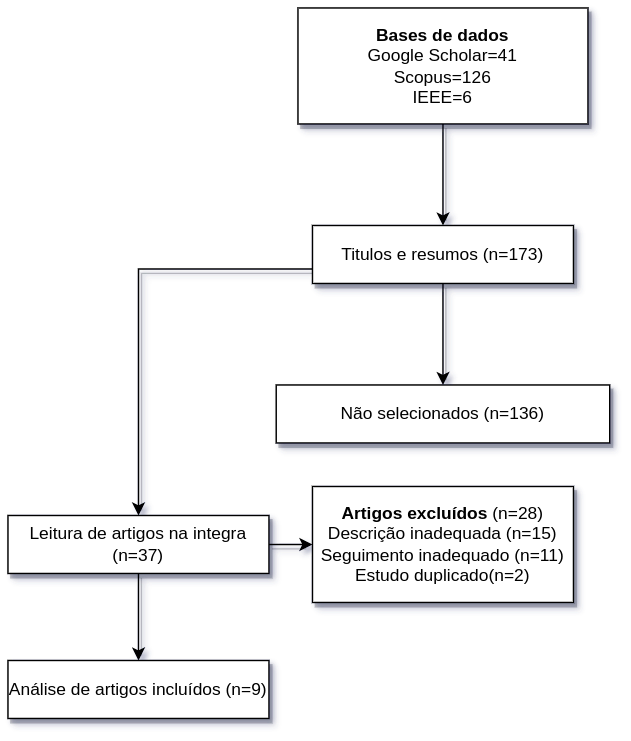
\includegraphics[height=4.5in]{recursos/imagens/project/revisao_panoptica.png}
%     \label{project:revision:fig:1}

%     Fonte: do próprio autor.
% \end{figure}

% Desse modo, com base na revisão bibliográfica conduzida, apenas um conjunto seleto de X itens foram escolhidos para a complementação do estudo em questão. Esses itens são destacados na Figura \ref{project:revision:fig:1} e listados em detalhes na Tabela \ref{project:revision:tab:1}.


% \begin{table}[H]
%     \centering
%     \caption{Trabalhos selecionados a partir da revisão sobre segmentação panóptica.}
%     \label{project:revision:tab:1}
%     \resizebox{\textwidth}{!}{
%     \begin{tabular}{l|l}
%         \textbf{Título}                                                &  \textbf{Referência}    \\ \hline
%         Part-Aware Panoptic Segmentation                               &  \cite{DeGeus2021}      \\
%         Improving Panoptic Segmentation at All Scales                  &  \cite{Porzi2021}       \\
%         SpatialFlow: Bridging All Tasks for Panoptic Segmentation      &  \cite{Chen2019a}       \\
%         Visual relation of interest detection based on part detection  &  \cite{YouZhou2021}     \\
%         Panoptic Image Annotation with a Collaborative Assistant       &  \cite{Jasper2020}      \\
%         Panoptic Segmentation-Based Attention for Image Captioning     &  \cite{Cai2020}         \\
%         Supplementary Material: Part-aware Panoptic Segmentation       &  \cite{DeGeus2021a}     \\
%         Panoptic Segmentation: A Review                                &  \cite{Elharrouss2021}  \\
%         PartImageNet: A Large, High-Quality Dataset of Parts           &  \cite{He2021}   
%     \end{tabular}}

%     \vspace*{1 cm}
%     Fonte: do próprio autor.
% \end{table}


\subsection{Considerações Finais do Capítulo}
\label{project:final}
 Este capítulo abordou várias facetas do projeto, proporcionando uma compreensão aprofundada da metodologia adotada e dos procedimentos experimentais realizados. Inicialmente, a seção de materiais e métodos ofereceu uma descrição detalhada das tecnologias e do hardware que foram necessários para implementar e executar as arquiteturas de redes neurais. Apresentou também o conjunto de dados utilizados, o conceito de transferência de aprendizagem e o processo de aumento de dados nos problemas explorados pelo projeto, com o intuito de evidenciar os benefícios do método proposto (BPCAPooling) e as alterações resultantes na camada de \textit{pooling} em diferentes arquiteturas de redes. Precisamente, todas essas descrições foram cruciais para estabelecer o contexto adequado para a pesquisa realizada.

A Metodologia Experimental, por sua vez, aprofundou-se na seleção das métricas para avaliar o desempenho dos modelos, com uma distinção clara entre as métricas associadas a problemas de classificação e aquelas relacionadas a desafios de segmentação semântica. Foi elucidado, também, sobre as configurações dos parâmetros de treinamento e de teste. Outrossim, esta seção enfocou na explicabilidade dos modelos, apresentado o uso de ferramentas do âmbito da Inteligência Artificial Explicável (XAI) para tornar os modelos de aprendizado profundo mais transparentes.

% Finalmente, na seção de Revisão de Literatura, vários trabalhos relevantes no campo de classificação de imagem e segmentação semântica foram discutidos, oferecendo uma visão compreensiva da dinâmica atual da pesquisa nesse campo.

Com isso, espera-se que este capítulo tenha fornecido uma visão clara e completa da metodologia adotada nesta pesquisa, propiciando assim um arcabouço sólido para as análises subsequentes dos resultados experimentais obtidos, que serão detalhados no próximo capítulo.